\chapter{Questionnaire for user segmentation}
This chapter anwers the Research Question \textbf{RQ 2: Which criteria do questions have to meet, that shall identify the type of a user?}


In the State of the Art chapter the User Segmentation \ref{chap:usersegmentation} from Smart Cities Demo Aspern on which this thesis builds up upon is explained. With regard to the Paper Prototyping session we need users that clearly can be allocated to a user segment. To find users for each user segment we created a questionnaire. The user survey leaned on to the first questionnaire of the quantitative study of Aspern Smart City Research. The original questionnaire of ASCR comprised of 48 questions. The factor analysis of the returned questionnaire identified the four dimensions: Comfort-centred, Technology-centred, Data Sensibility and Living in Seestadt. The following cluster analysis found out four segments. For the definition of the segments only two of the four factors were relevant for describing the characteristics of a user group. For our study we focused on these two factors which are the comfort and the technology orientation. So, we took all the questions of the original questionnaire which answers were identified by the cluster analysis to be significant for the user segmentation. Out of the 48 questions of the original questionnaire ten were relevant for allocating a user to a user segment.

For creating and sending the survey we used Google Forms. As the motivation to find subjects who complete a survey increases as the question difficulty increases \cite{andrews2007conducting}, our questionnaire only comprised of ten questions and the average time for answering the whole questionnaire only took one minute. We sent the questionnaire to 57 people, trying to have a good distribution of different ages, educational levels, jobs and interests. 41 questionnaires were returned.

For evaluating the response we used Google Spreadsheet and Microsoft Excel. The answers of each person was evaluated against the characteristics of each of the four user segments. Of course not every user could easily be assigned to exactly one user segment. For each user the correspondence to each of the four user segments was calculated and expressed in percent. The ones who had a clear correspondence of more than 50 \% to one user type were chosen as test users for the paper prototyping, the usability tests and the user study later on. So at least one user for each user type was chosen. 

Given the answer of the first research questions and the results of the survey we can give a conclusive answer to the following research question:

\textbf{RQ 2: Which criteria do questions have to meet, that shall identify the type of a user?}

The questions shall concern the main characteristics of every user type regarding the factors technology and comfort. This means the survey should include questions that:

\begin{itemize}
	\item check the interest in energy
	\item investigate the knowledge of the consumption of electric devices
	\item detect the importance of saving at energy costs
	\item determine whether a user programs from time to time
	\item find out if home automation possibilities are used
	\item examine the pattern of showering or taking a bath
	\item check the behaviour of switching out the light when leaving a room
	\item ask if the light is sometimes forgotten to be switched of when leaving the apartment
	\item ask for the preferred use of lighting 	
\end{itemize}

Additionally, the questions shall be short, comprehensive and easy to answer, as mentioned in~\ref{sec:survey}. The whole questionnaire can be found in ~\nameref{chap:appendixA}.


\section{Paper Prototype for proposed mobile application}

After having found test users for the paper prototyping workshop, the preparation for it began. As described before in \ref{section:paperprototyping} we follow the Step-by-Step guide of Arnowitz et al. \cite{arnowitz2010effective} to create a Paper Prototype.

The first task of the Step-by-Step guide is to define the tasks in a scenario narration.

	\subsection{Scenario narration}
	
	The main goal of the mobile application that shall be developed is to give eco-feedback. This feedback shall primarily focus on the consumption of electricity, water and heating and the emission of carbon-dioxide. So the history consumption rate of these data shall be available to look into. A comparison of the consumption during different time intervals shall also be possible. This comparison can be drawn to one's own consumption but also to a comparable household, to an average consumption rate of the neighbours, the city or the European Union. On a dashboard the current measured values, the consumption of the day and some current settings shall be shown. The management of the home automation system shall also be available via the app. Tips for saving money by saving energy shall also be given. Energy saving-tips shall be tailored to the characteristics of a user type. Especially for Hedonists the menu item "Project" will be interesting. Here projects are listed, which show possible further home automation items that can help at energy saving. A user can read frequently asked questions in the FAQ section.
	
	\subsection{Design and evaluation of Paper Prototypes}	
	Having in mind the above mentioned tasks we designed multiple versions of the paper prototypes that resulted from several runs through the Step-by-Step guide for the creation of a paper prototype of Arnowitz et al. \cite{arnowitz2010effective}. The design was done with the third research question in mind, that shall be answered with the paper prototypes.
	
	\textbf{RQ 3: What are the design possibilities when it comes to tailoring interfaces to a user segment in the scope of electricity consumption data?}
	
	The existing approaches of eco-feedback applications have been evaluated in the section~\ref{sec:approaches}. Especially the design principles were the basis for the hand-sketched drafts.
	
	 and analysing their approach of trying to change a user's behaviour. One application will be investigated in particular and will be the basis for the paper prototypes.
	
	\subitem{\textbf{Professionals}}: The user study revealed that Professionals have high interest in energy issues. As they are deep into the topic and prefer more detailed information in individual offers they can have a look on the energy consumption on a very detailed level, such as a consumption rate on a granularity of minutes. Professionals also should have a possibility within the application to compare energy consumptions of different time intervals. According to the user study Professionals also like to compare themselves to others. Professionals also like rationally justified explanations and instructions for use. Notifications should give tips on saving energy or CO2, give concrete instructions for use and provides deeper information in Energy topics. This results in the following tasks for professionals:
	

		
	\subitem{\textbf{Optimizer}}: Optimizer primarily aim at optimizing energy costs, so the app should give easy to find tips on how to save energy and therefore costs. Optimizers also prefer less time of interaction and rather like unclear instructions. Therefore the notifications also should give concrete instructions on how to save energy or CO2. Optimizer also like to know the concrete benefits of a certain behaviour change. The explanations shall be as close to reality as possible and technical language shall be avoided. The energy feedback is reduced to essential information and the detailed graphs for energy consumption that the Professionals get, should not be visible at a first glance for an Optimizer. The saved costs after a behaviour change shall also be visible to provide some kind of reward for the new habits. For Optimizer also trouble shooting shall be easily accessible, in order to reduce the time they are spending with the application and not to loose them on the way.
	

	
	\subitem{\textbf{Indifferents}}:
	The Indifferents have low interest in energy topics in general, so the main requirement of the application for this type of user is in the first run to sensitize them for the topic, to raise awareness and to make electricity and CO2 saving appealing to them. To awaken their interest for energy and sustainability a gamification approach will be used. For opening the application once a day the user earns points. Points are also earned for clicking on notifications and reading the article. Tips for saving energy or CO2 should not concern longer usage of laptops or entertainment screens, as streaming and use of social media is an important leisure activity for Indifferents.
	

	\subitem{Hedonists}:
	The youngest segment, the Hedonists, are keen on developing technical solutions. The interest in technology can be used to give instructions for programming technical devices and using home automation. The primary motive for the Hedonists is not to save energy but the interest in technology. This will be considered in the notifications and tips of the day. The hedonistic lifestyle with its strong convenience and comfort orientation is in the foreground. For a hedonist the comfort gain is of great relevance. Programming and establishing home automation aspects is a great interface between the aim of saving energy and the affinity of technology.
	

		el be shown in a dashboard, in about how much electricity, water and heating a user consumed, how much carbon-dioxide was produced and how the values can be made better in the sense of reducing consumptions. The screens shall be adapted to the user type to make the information and tips more attractive to a user's interests. The interfaces shall be different for each user but every user should basically have the possibility to do all tasks.
	
	\begin{enumerate}
		\item As a user I want to have a look on your consumption rate of the last day/week/month/year
		\item Compare your consumption rate of the last day/week/month/year with the consumption rate of the same week one year earlier.
		\item Compare your consumption rate of the last week with the average consumption rate of your neighbours
		\item Find tips on how to save more energy
		\item Find out what to do to save costs for electricity
		\item Find out how much you have saved in the last week
		\item Earn trophies by interacting with the App
		\item Start a project to install a home automation gadget that saves energy in the long run
		\item Report a problem
	\end{enumerate}
	
	
	
In order to elicit the requirements for the graphical user interfaces and to find usability mistakes we make use of Paper Prototyping. 



\section{Design Guidelines for tailoring interfaces to user segments}


\textit{Hedonists}:


Guideline 1: Adapt navigation drawer to requirements of user type

Description: Sort the items of the navigation drawer differently and adapt them for each user type

Effect:

Upside:

Downside:

Issues:

Background:

Guideline 2: Adapt navigation drawer to requirements of user type

Guideline 3: Adapt navigation drawer to requirements of user type

Preferred measurements
	Use Euro rather than kWh as measurement unit for Optimizer and Indifferents
	Use kWh rather than Euro as measurement unit for Professionals and Hedonists


Primary use case for app
	Professionals primarily use the app for monitoring their consumption rate
	Optimizer primarily use the app for saving purposes/Present primarily saving possibilities for Optimizer
	Indifferents primarily use the app because it makes fun (gamification character) Indifferents are interested in energy saving tips more if they can success in the game
	Hedonists' primary use case for the app is home automation

Communication
	Hedonists prefer praise 
	Use concrete instruction for Optimizer and avoid detailed information/Optimizer prefer concrete instructions to detailed information

Trouble Shooting
	Present a hotline for trouble shooting for optimizer/Optimizer prefer calling when an error occurs
	Present FAQs before telephone number for Hedonists and Indifferents and Professionals

Energy-saving
	Hedonists prefer to do projects that save energy for them in the long run
	Hedonists are comfort-oriented Do not present energy saving tips to Hedonists when they limit comfort
	Professionals are interested in deeper information for saving tips
	Professionals do not see gamification approaches as a motivation for saving energy tips
	Optimizer want to know how much they can save by following an Energy-saving tip
	Indifferents woul






 




\begin{figure}[h]
	\centering
	\begin{subfigure}[b]{0.24\columnwidth}
		\centering
		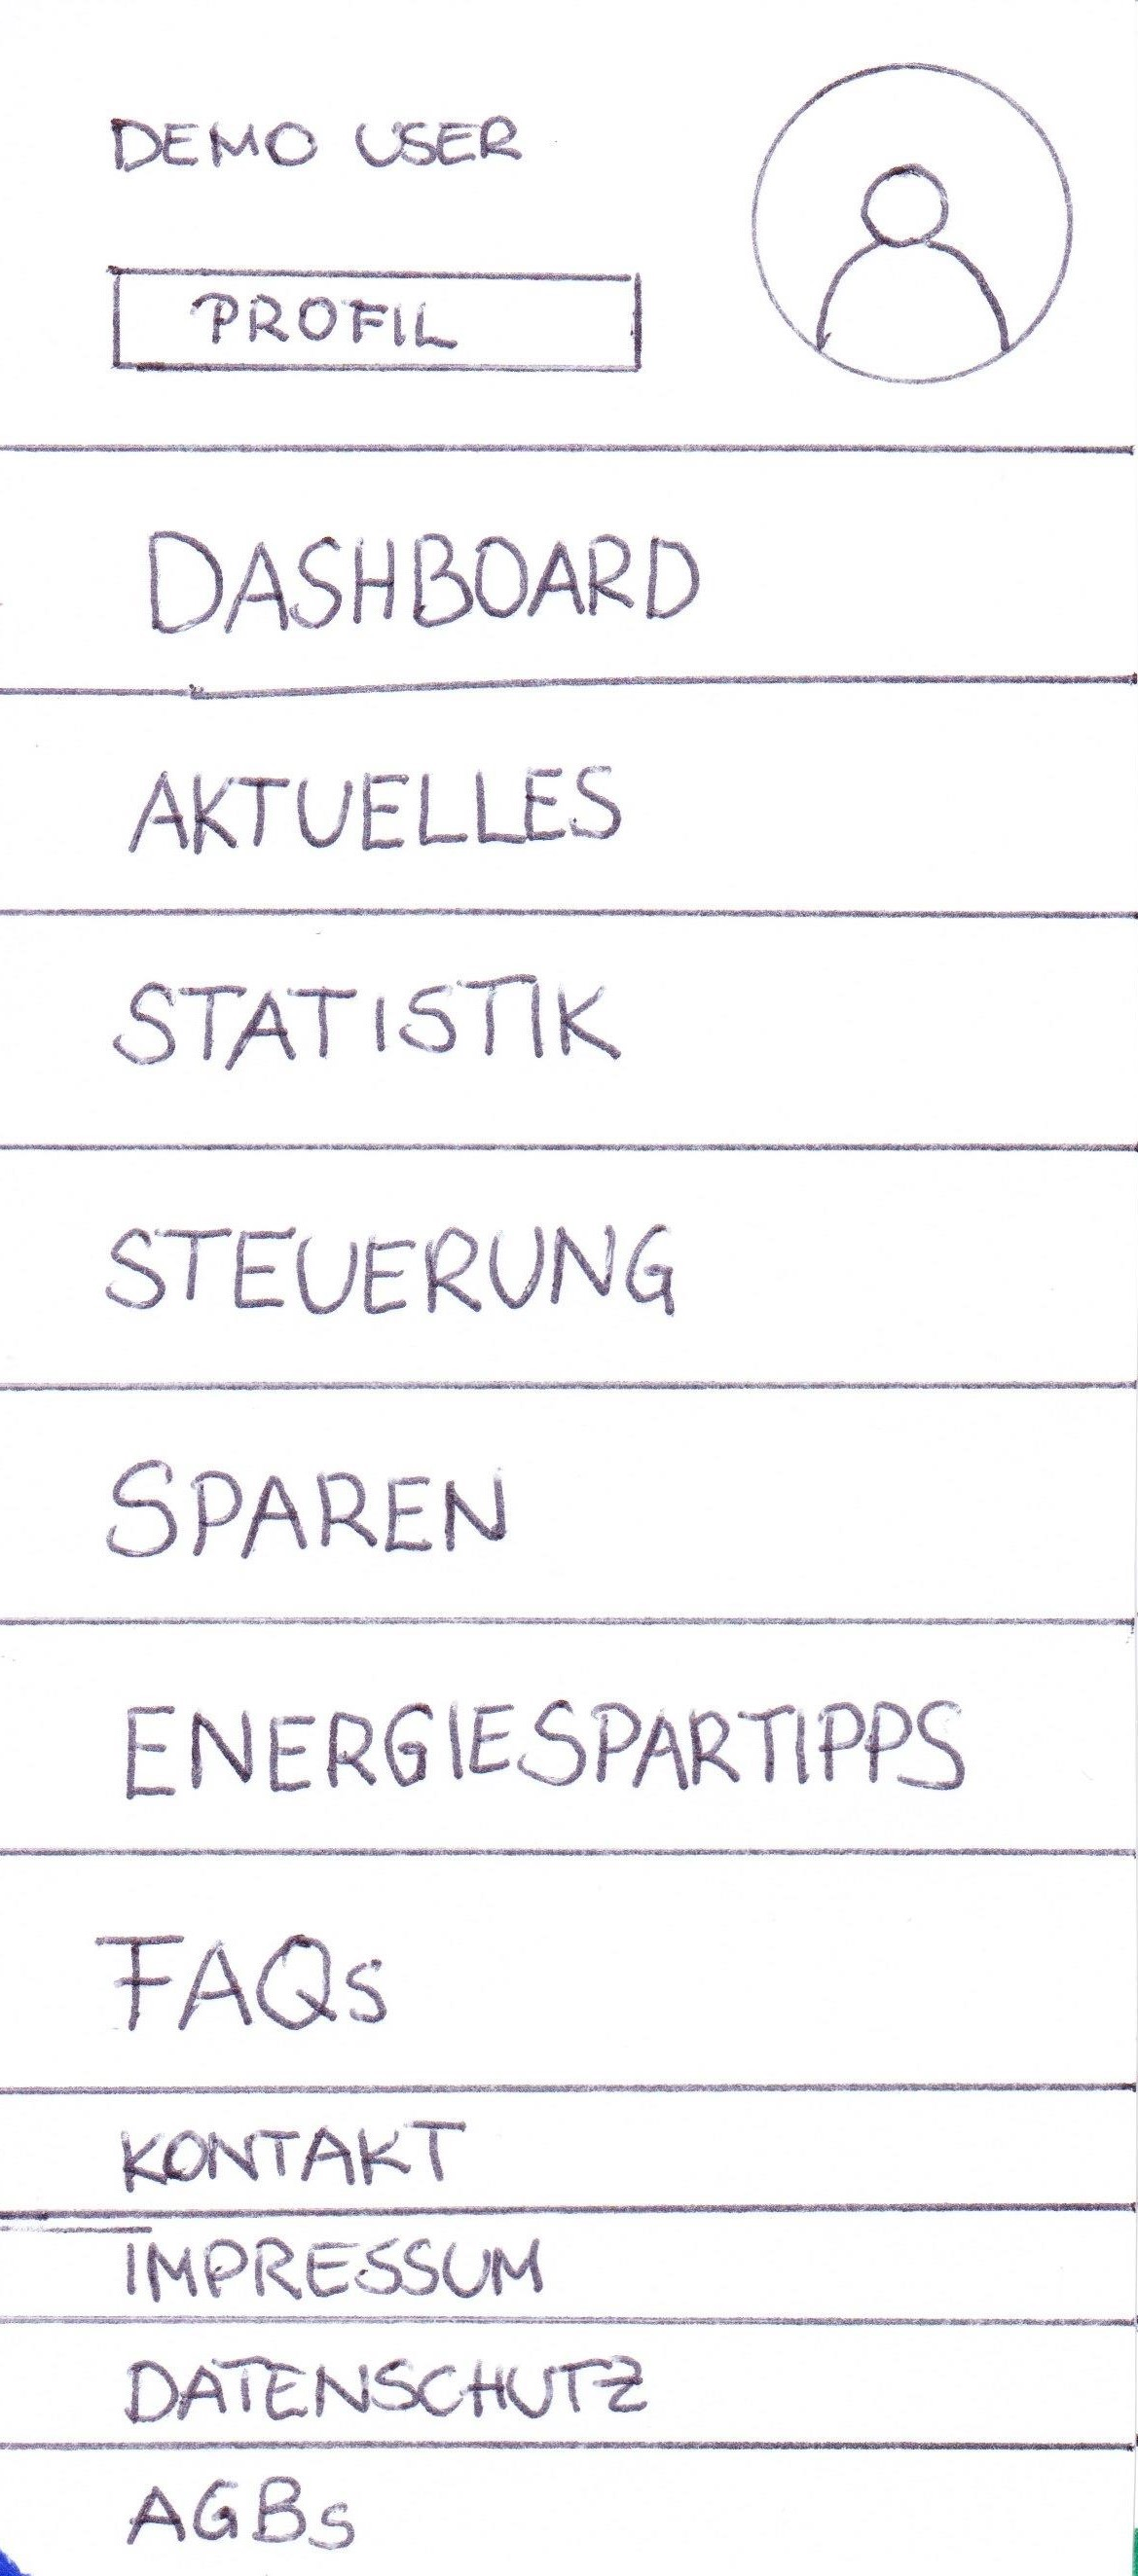
\includegraphics[width=\textwidth]{screens/drawer_1}
		\subcaption{Professional}
		\label{fig:drawer:professional}
	\end{subfigure}
	\begin{subfigure}[b]{0.24\columnwidth}
		\centering
		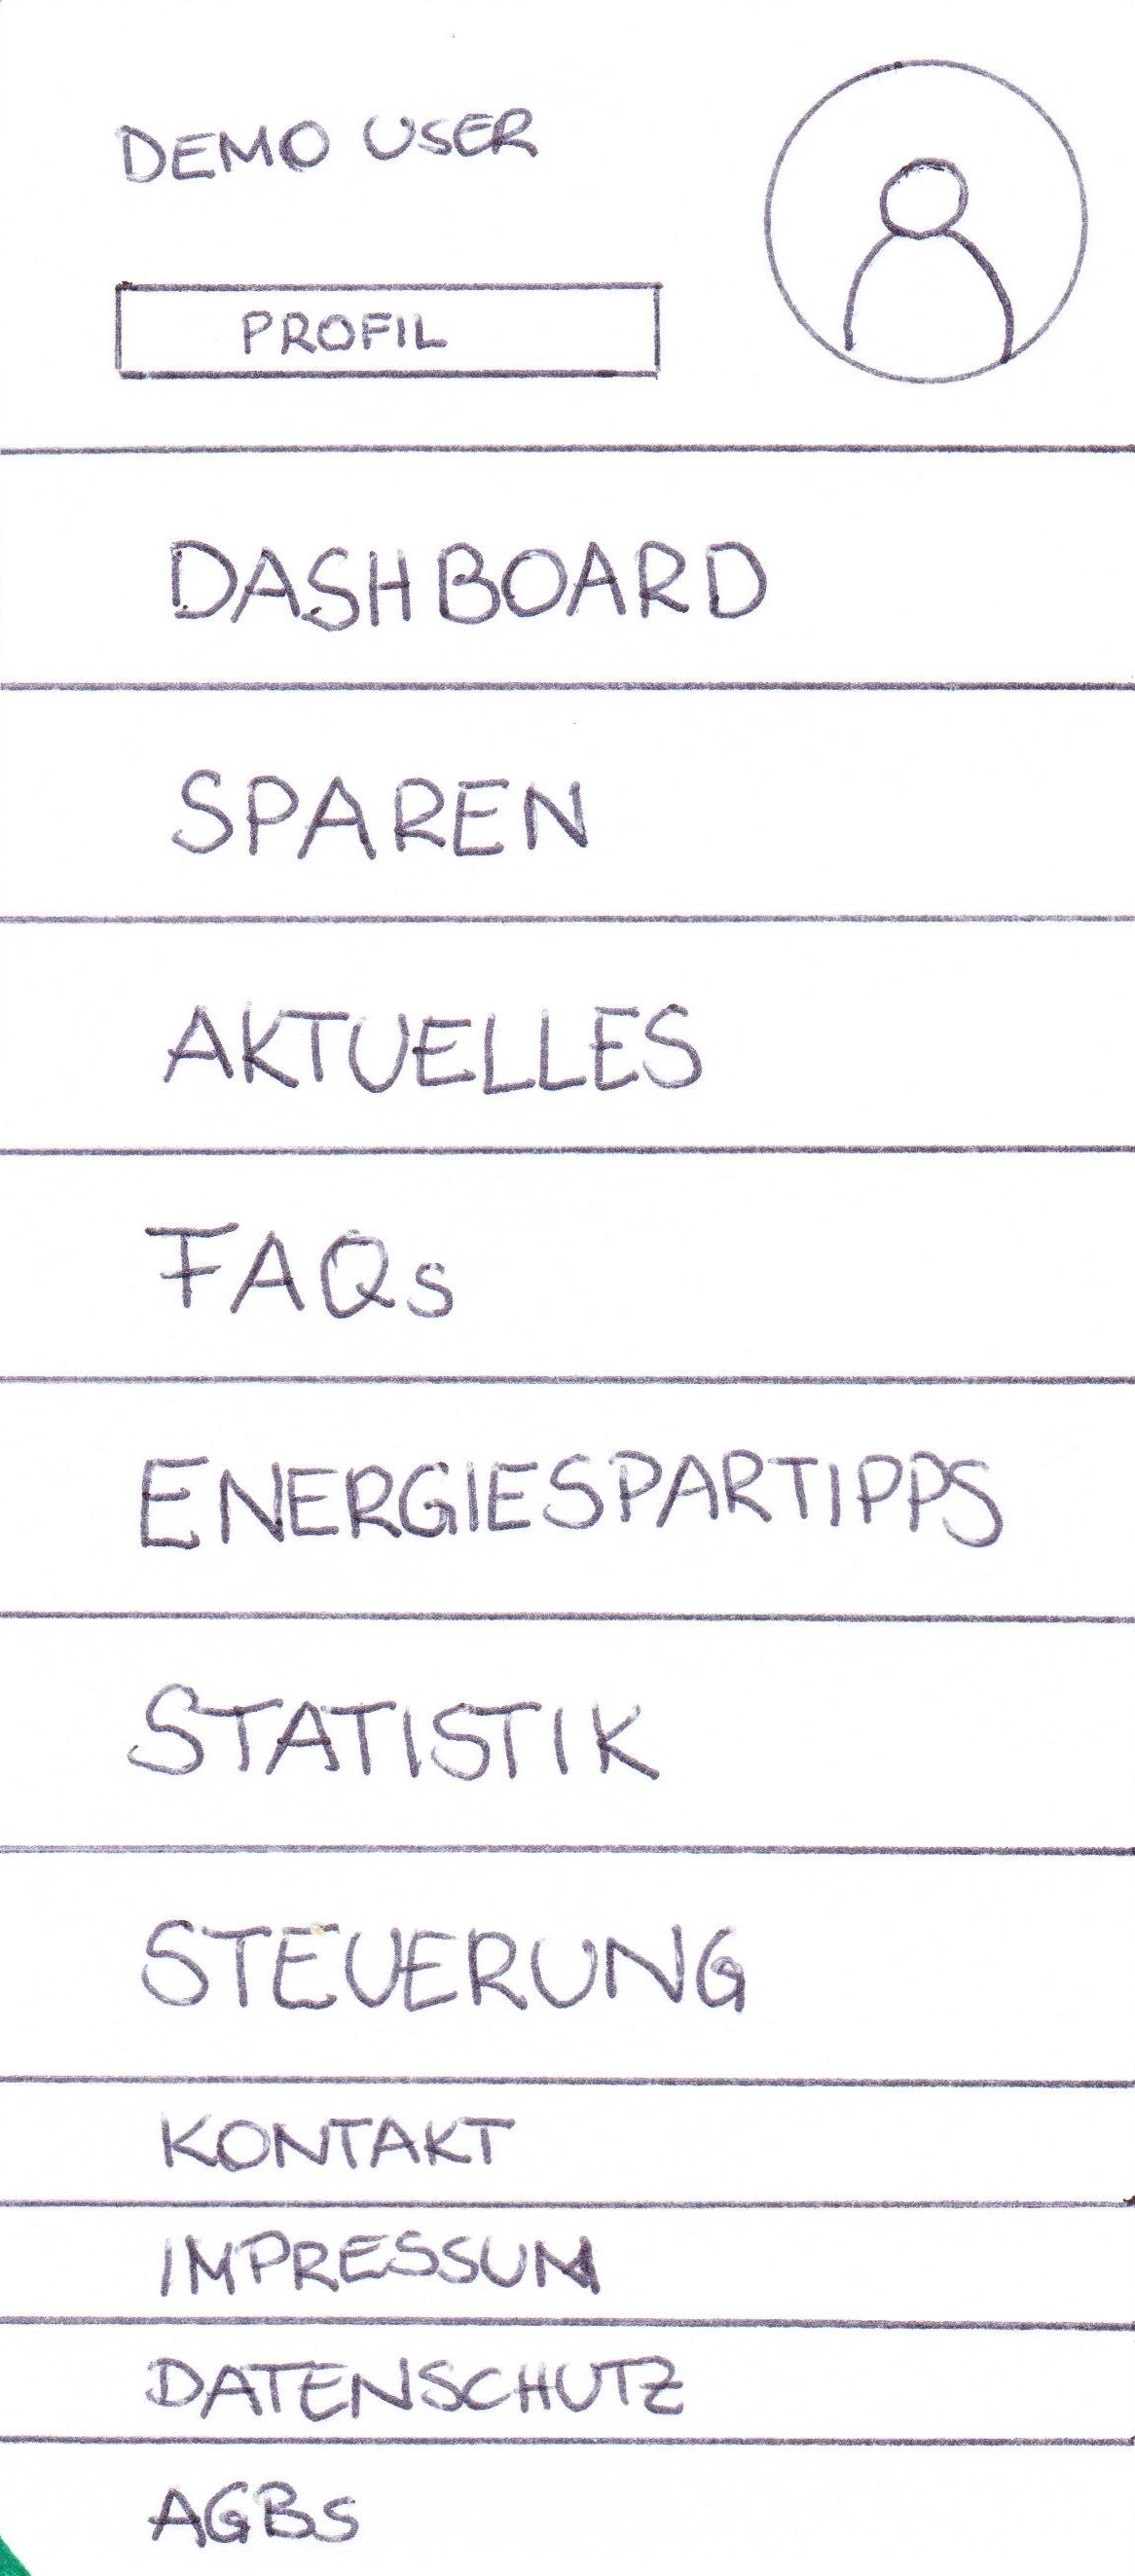
\includegraphics[width=\textwidth]{screens/drawer_2}
		\subcaption{Optimizer}
		\label{fig:drawer:optimizer}
	\end{subfigure}
	\begin{subfigure}[b]{0.24\columnwidth}
		\centering
		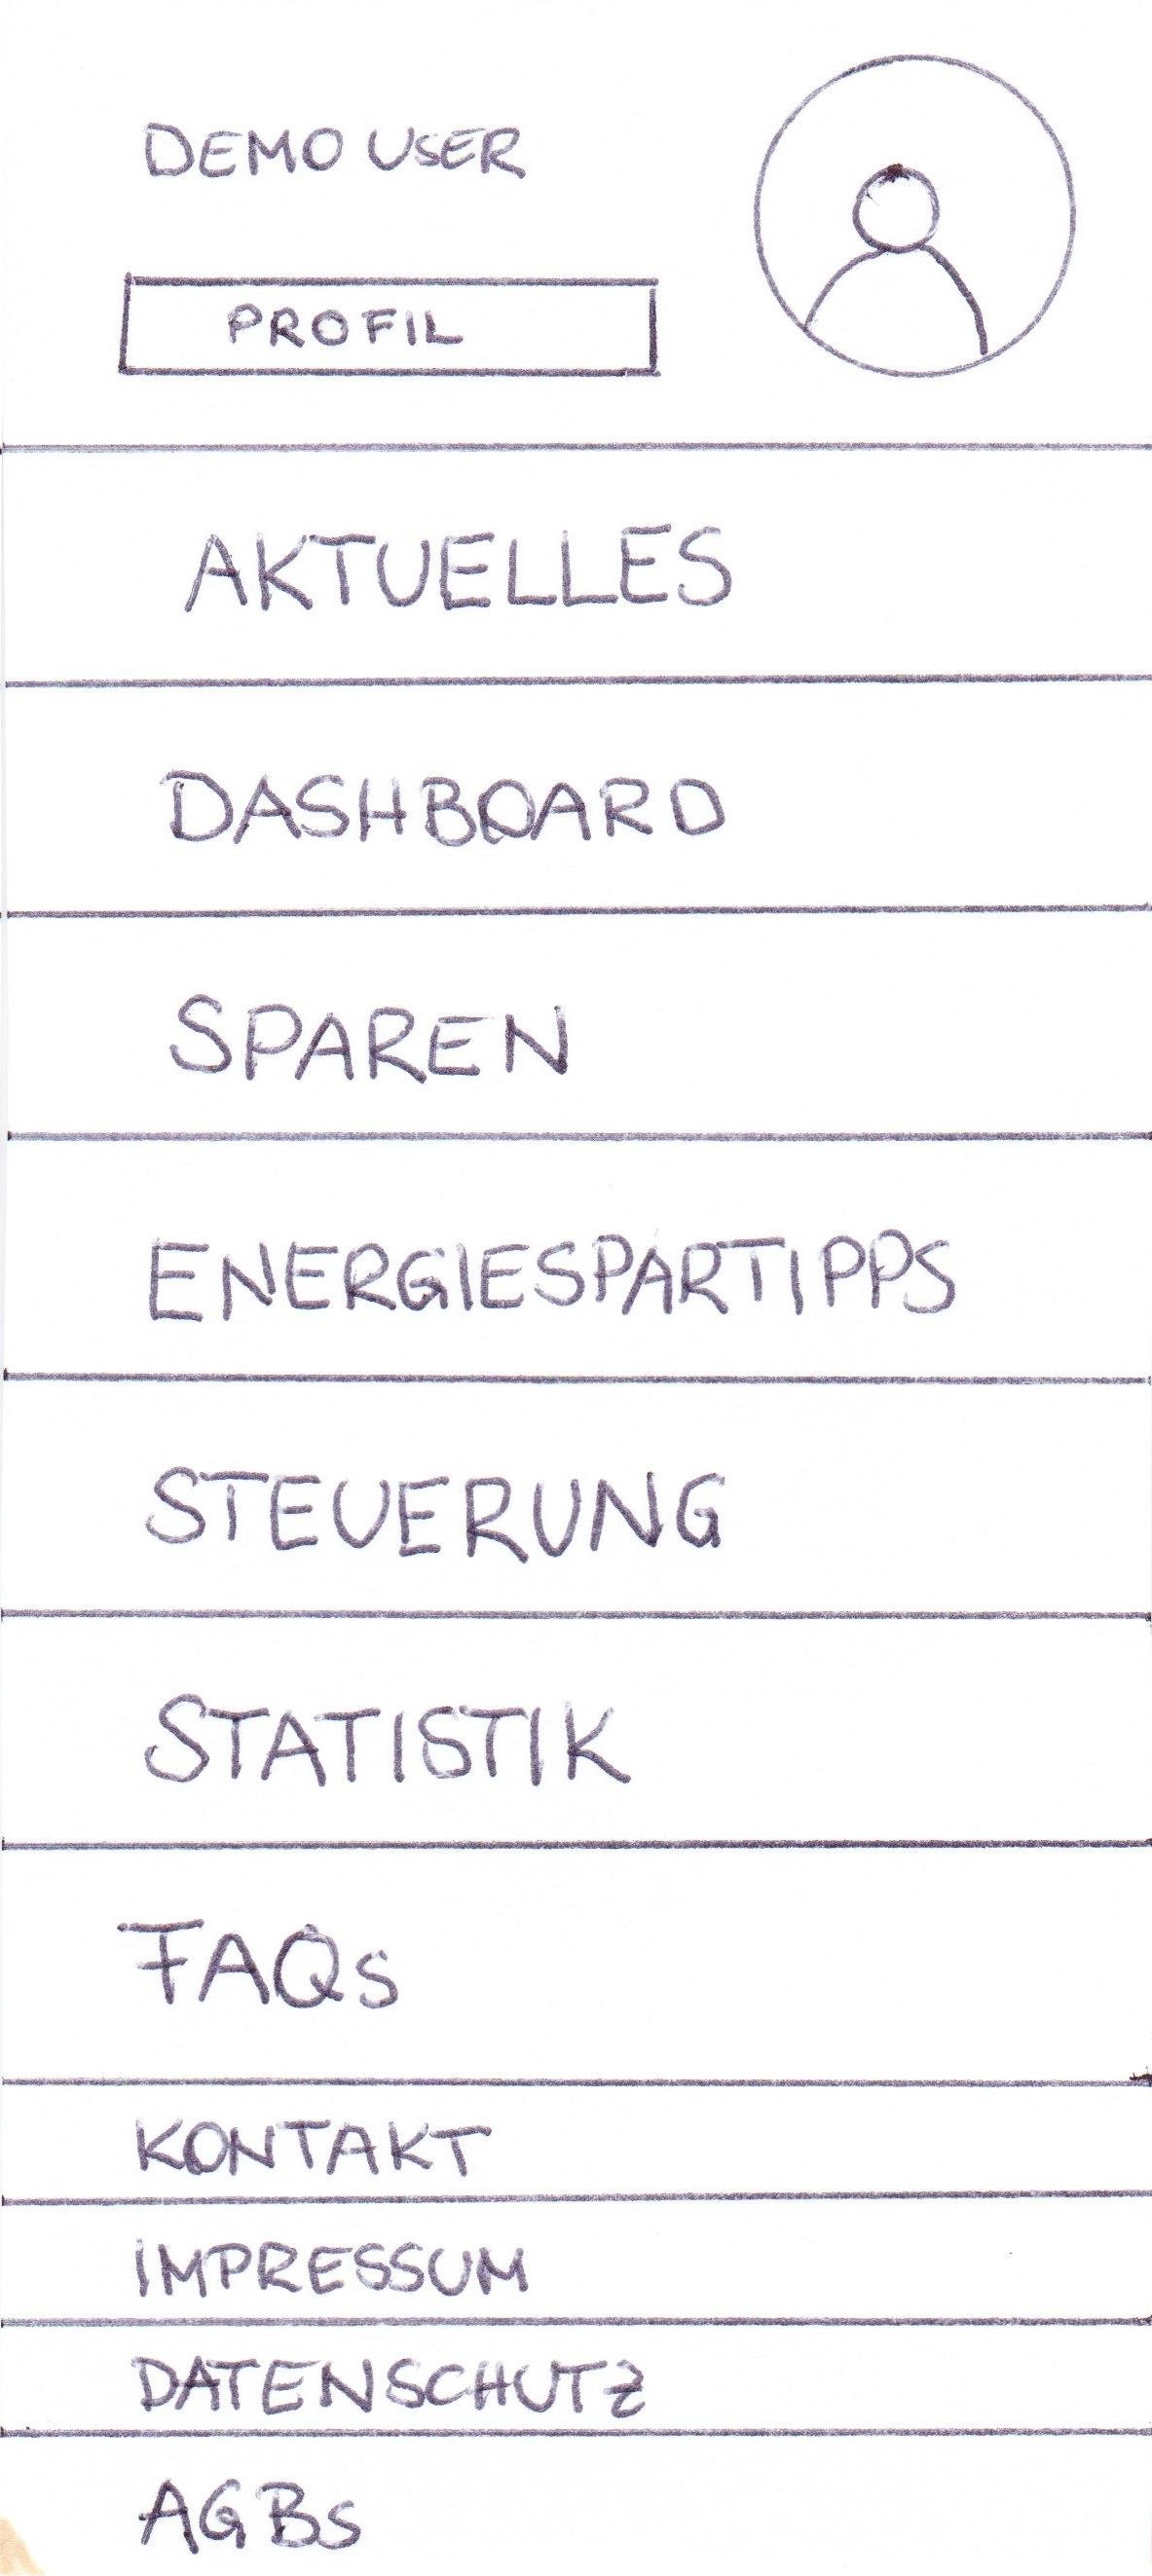
\includegraphics[width=\textwidth]{screens/drawer_3}
		\subcaption{Indifferent}
		\label{fig:drawer:indifferent}
	\end{subfigure}
	\begin{subfigure}[b]{0.24\columnwidth}
		\centering
		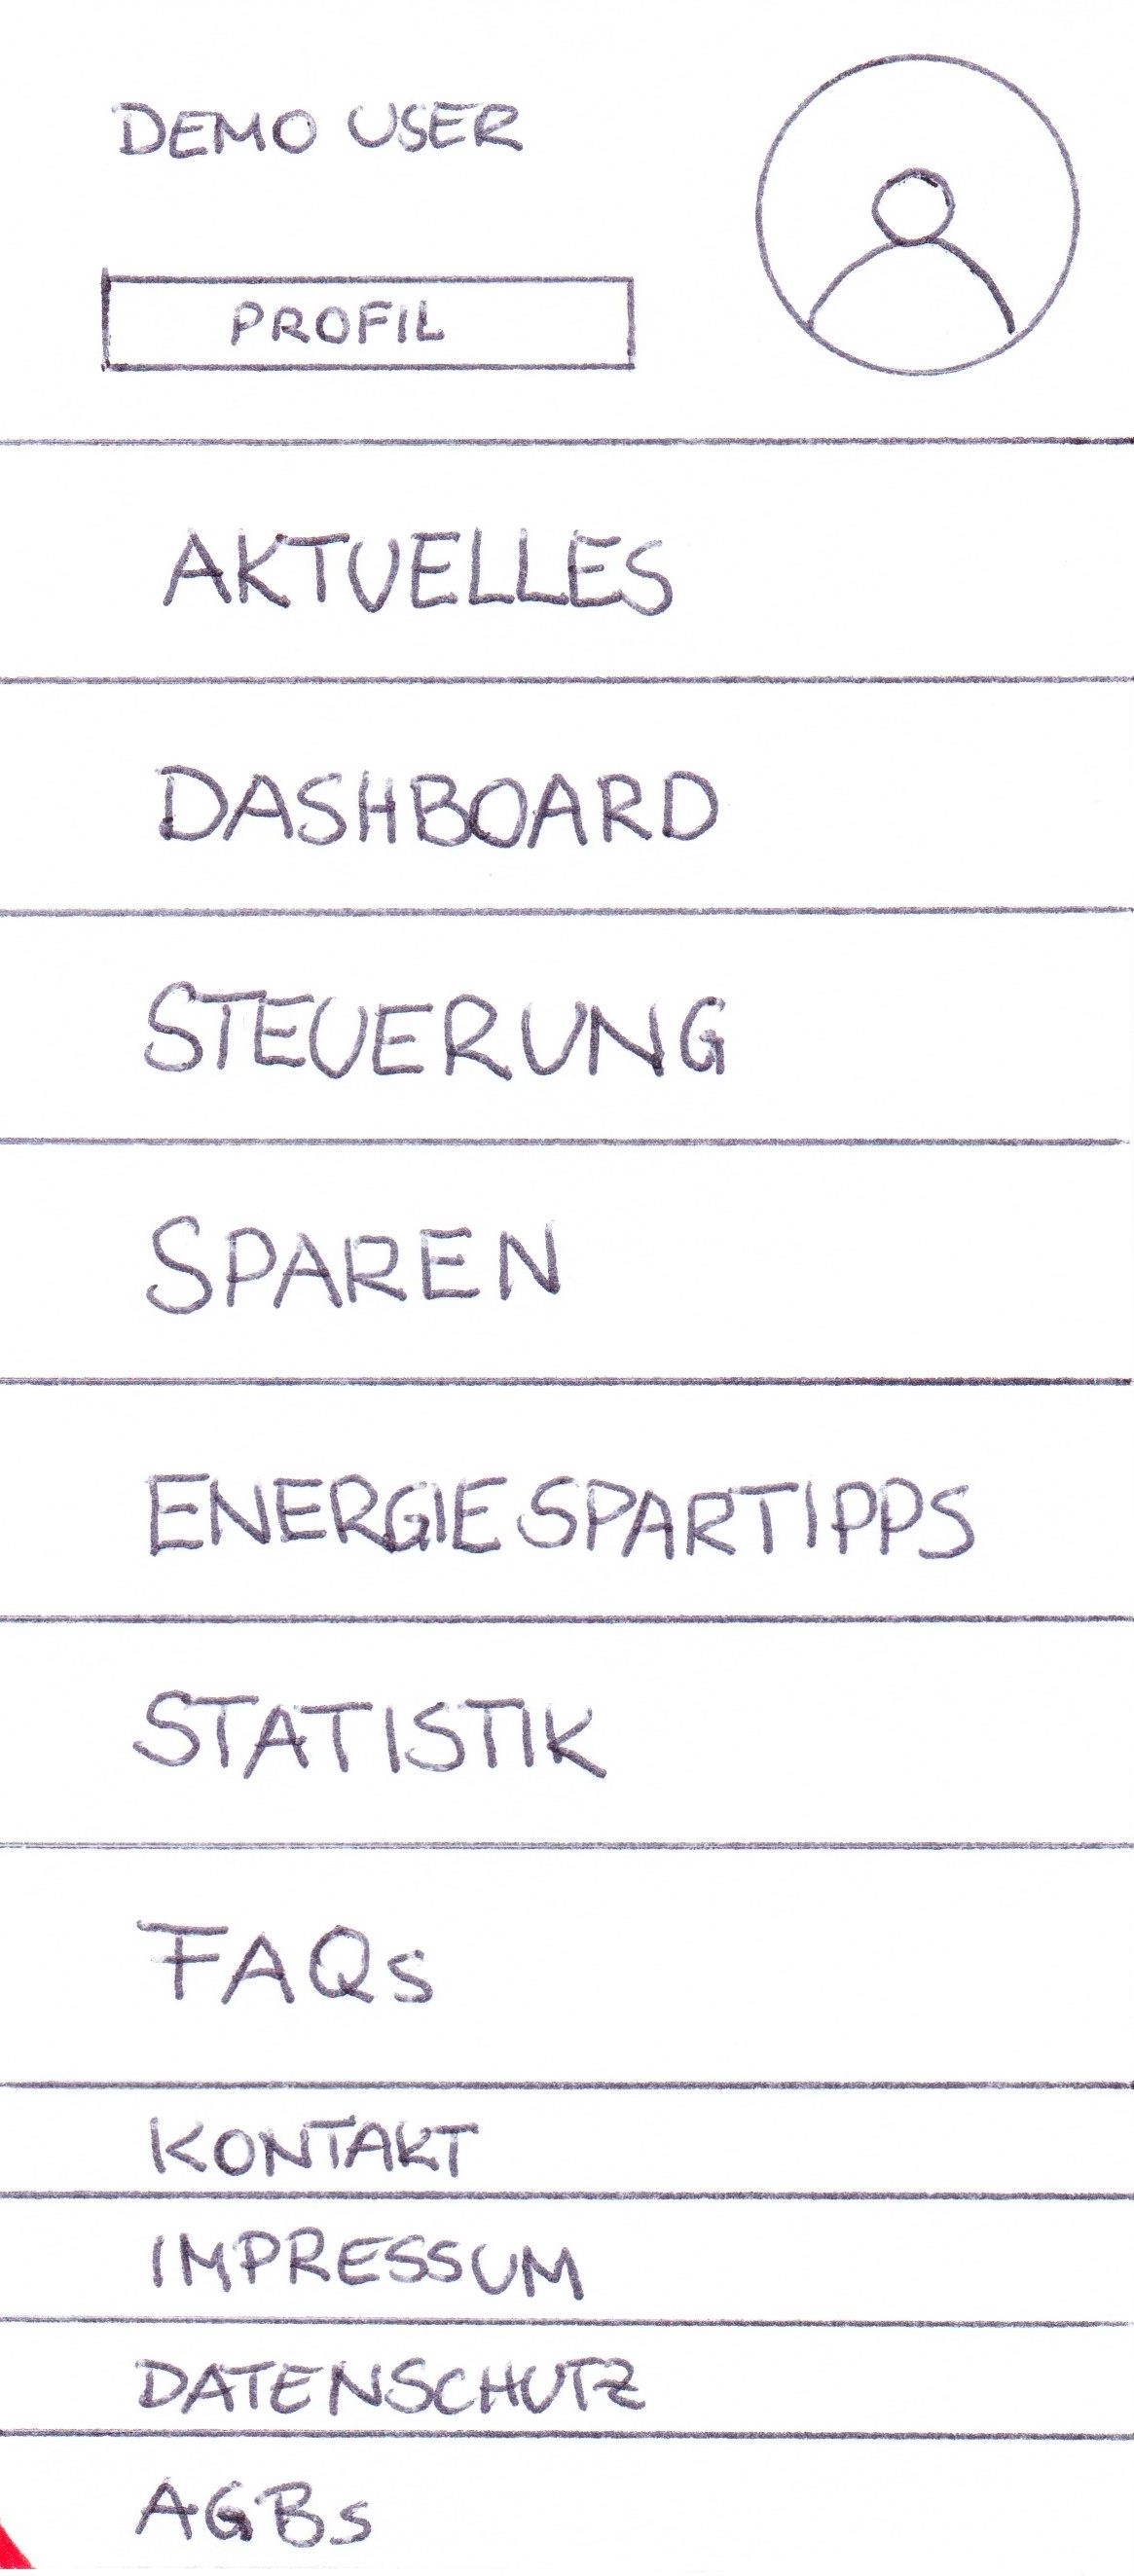
\includegraphics[width=\textwidth]{screens/drawer_4}
		\subcaption{Hedonist}
		\label{fig:drawer:hedonist}
	\end{subfigure}
	\caption{The proposed screen for the navigation drawer}
	\label{fig:drawer} % \label has to be placed AFTER \caption (or \subcaption) to produce correct cross-references.
\end{figure}

\begin{figure}[h]
	\centering
	\begin{subfigure}[b]{0.24\columnwidth}
		\centering
		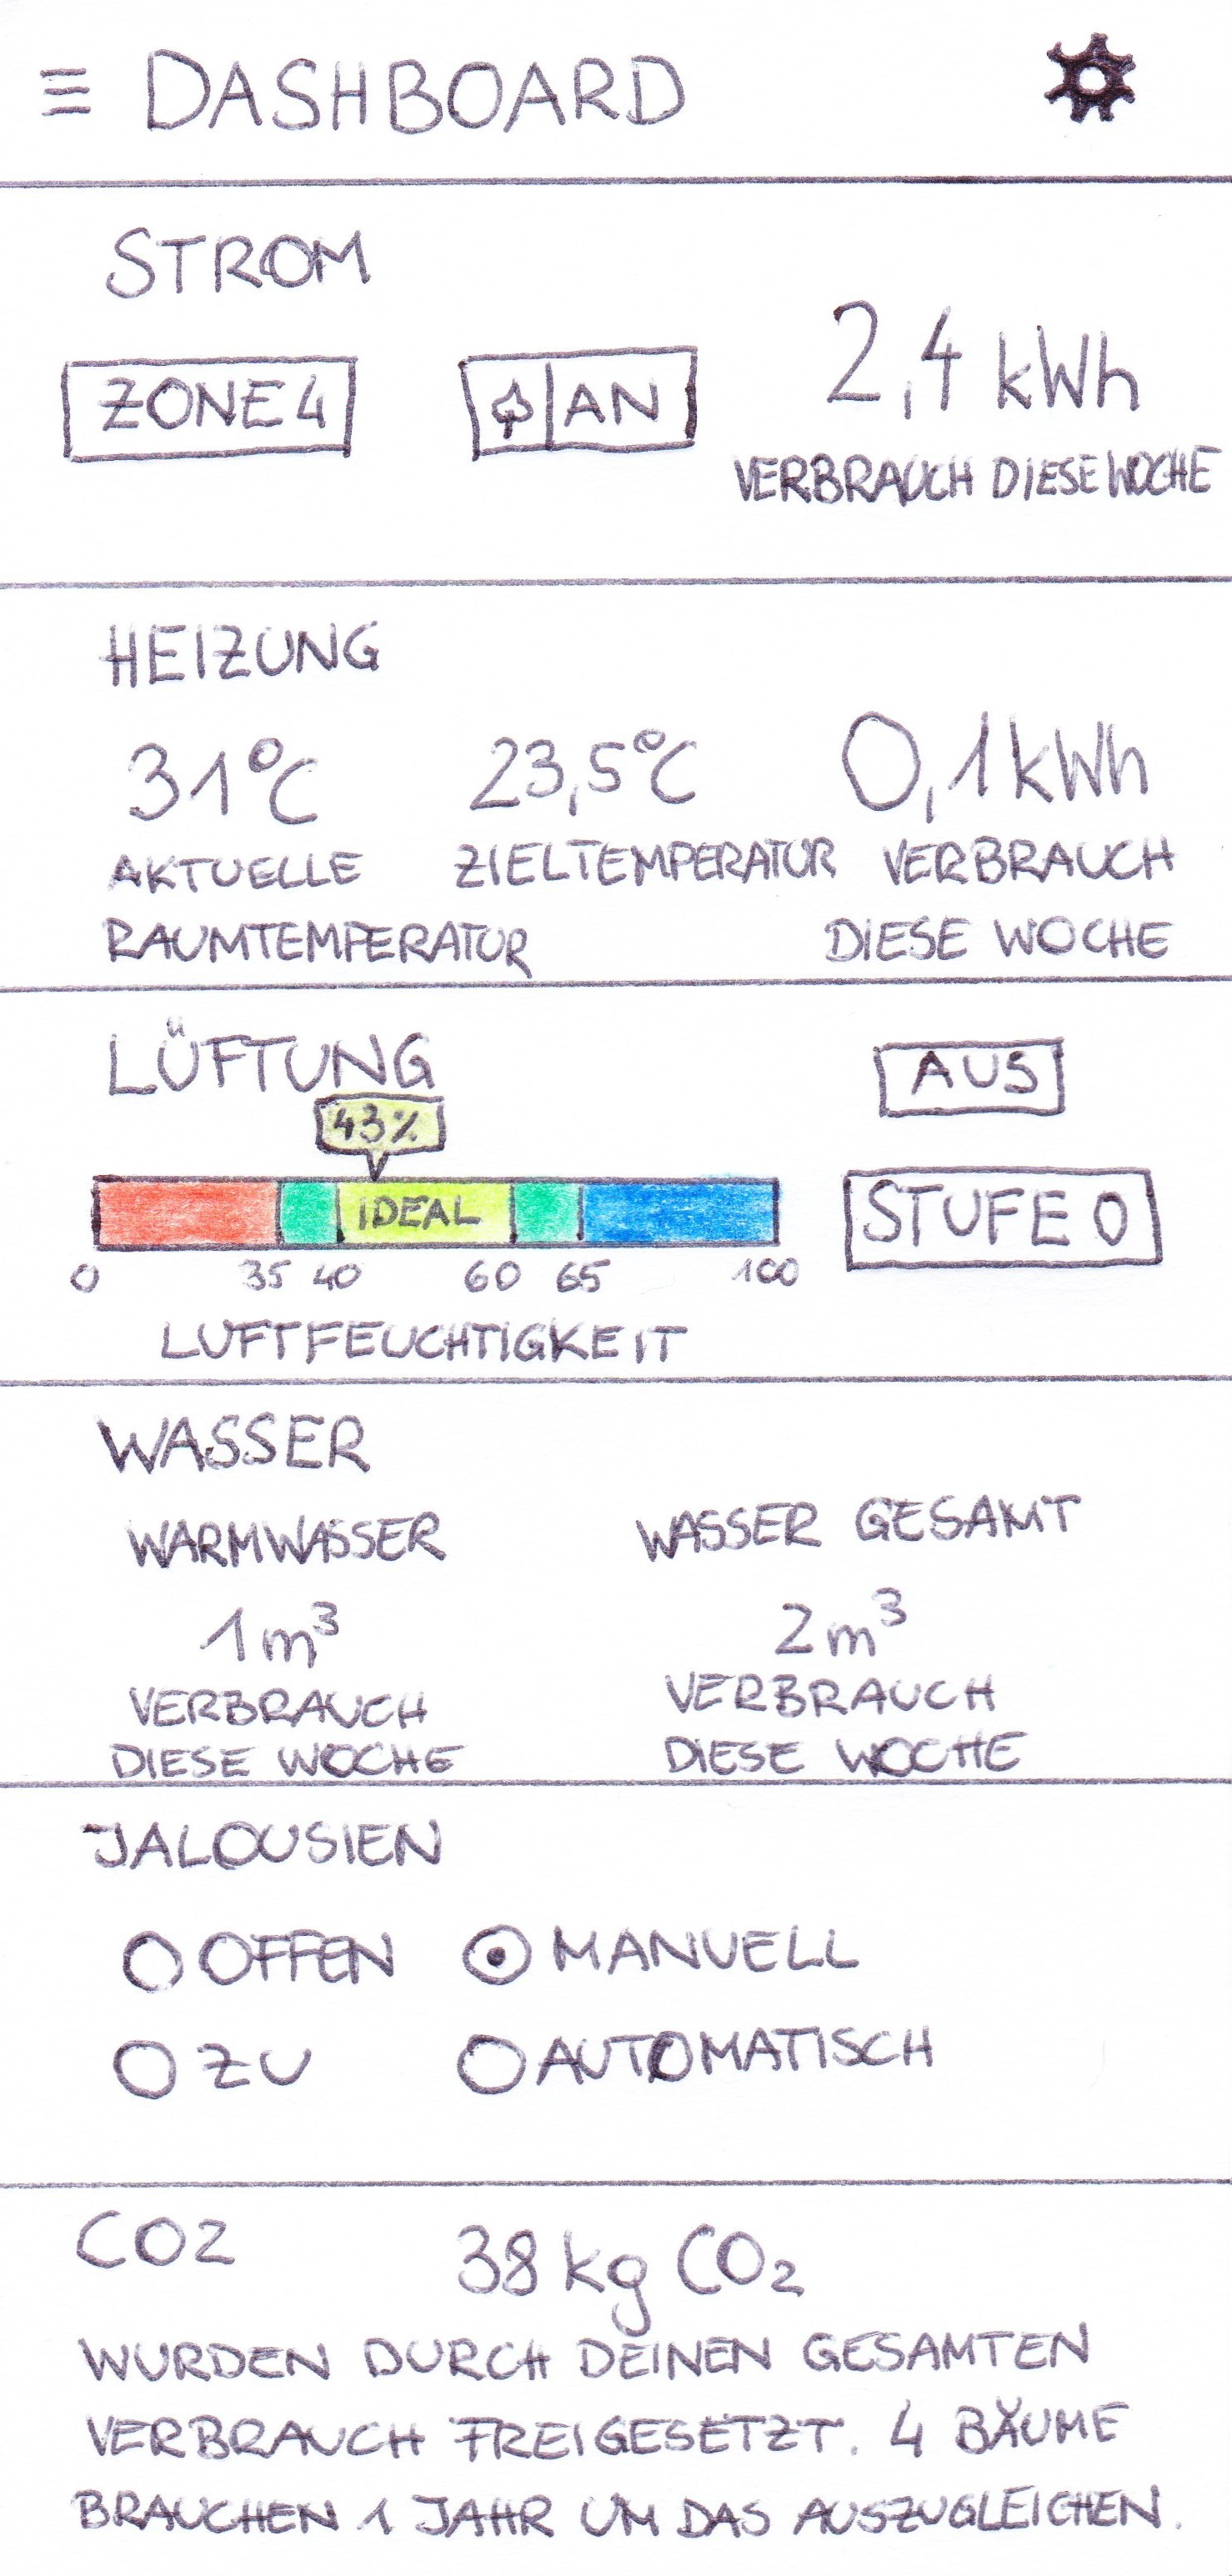
\includegraphics[width=\textwidth]{screens/dashboard_14}
		\subcaption{Professional and Hedonist}
		\label{fig:dasboard:professional}
	\end{subfigure}
	\begin{subfigure}[b]{0.24\columnwidth}
		\centering
		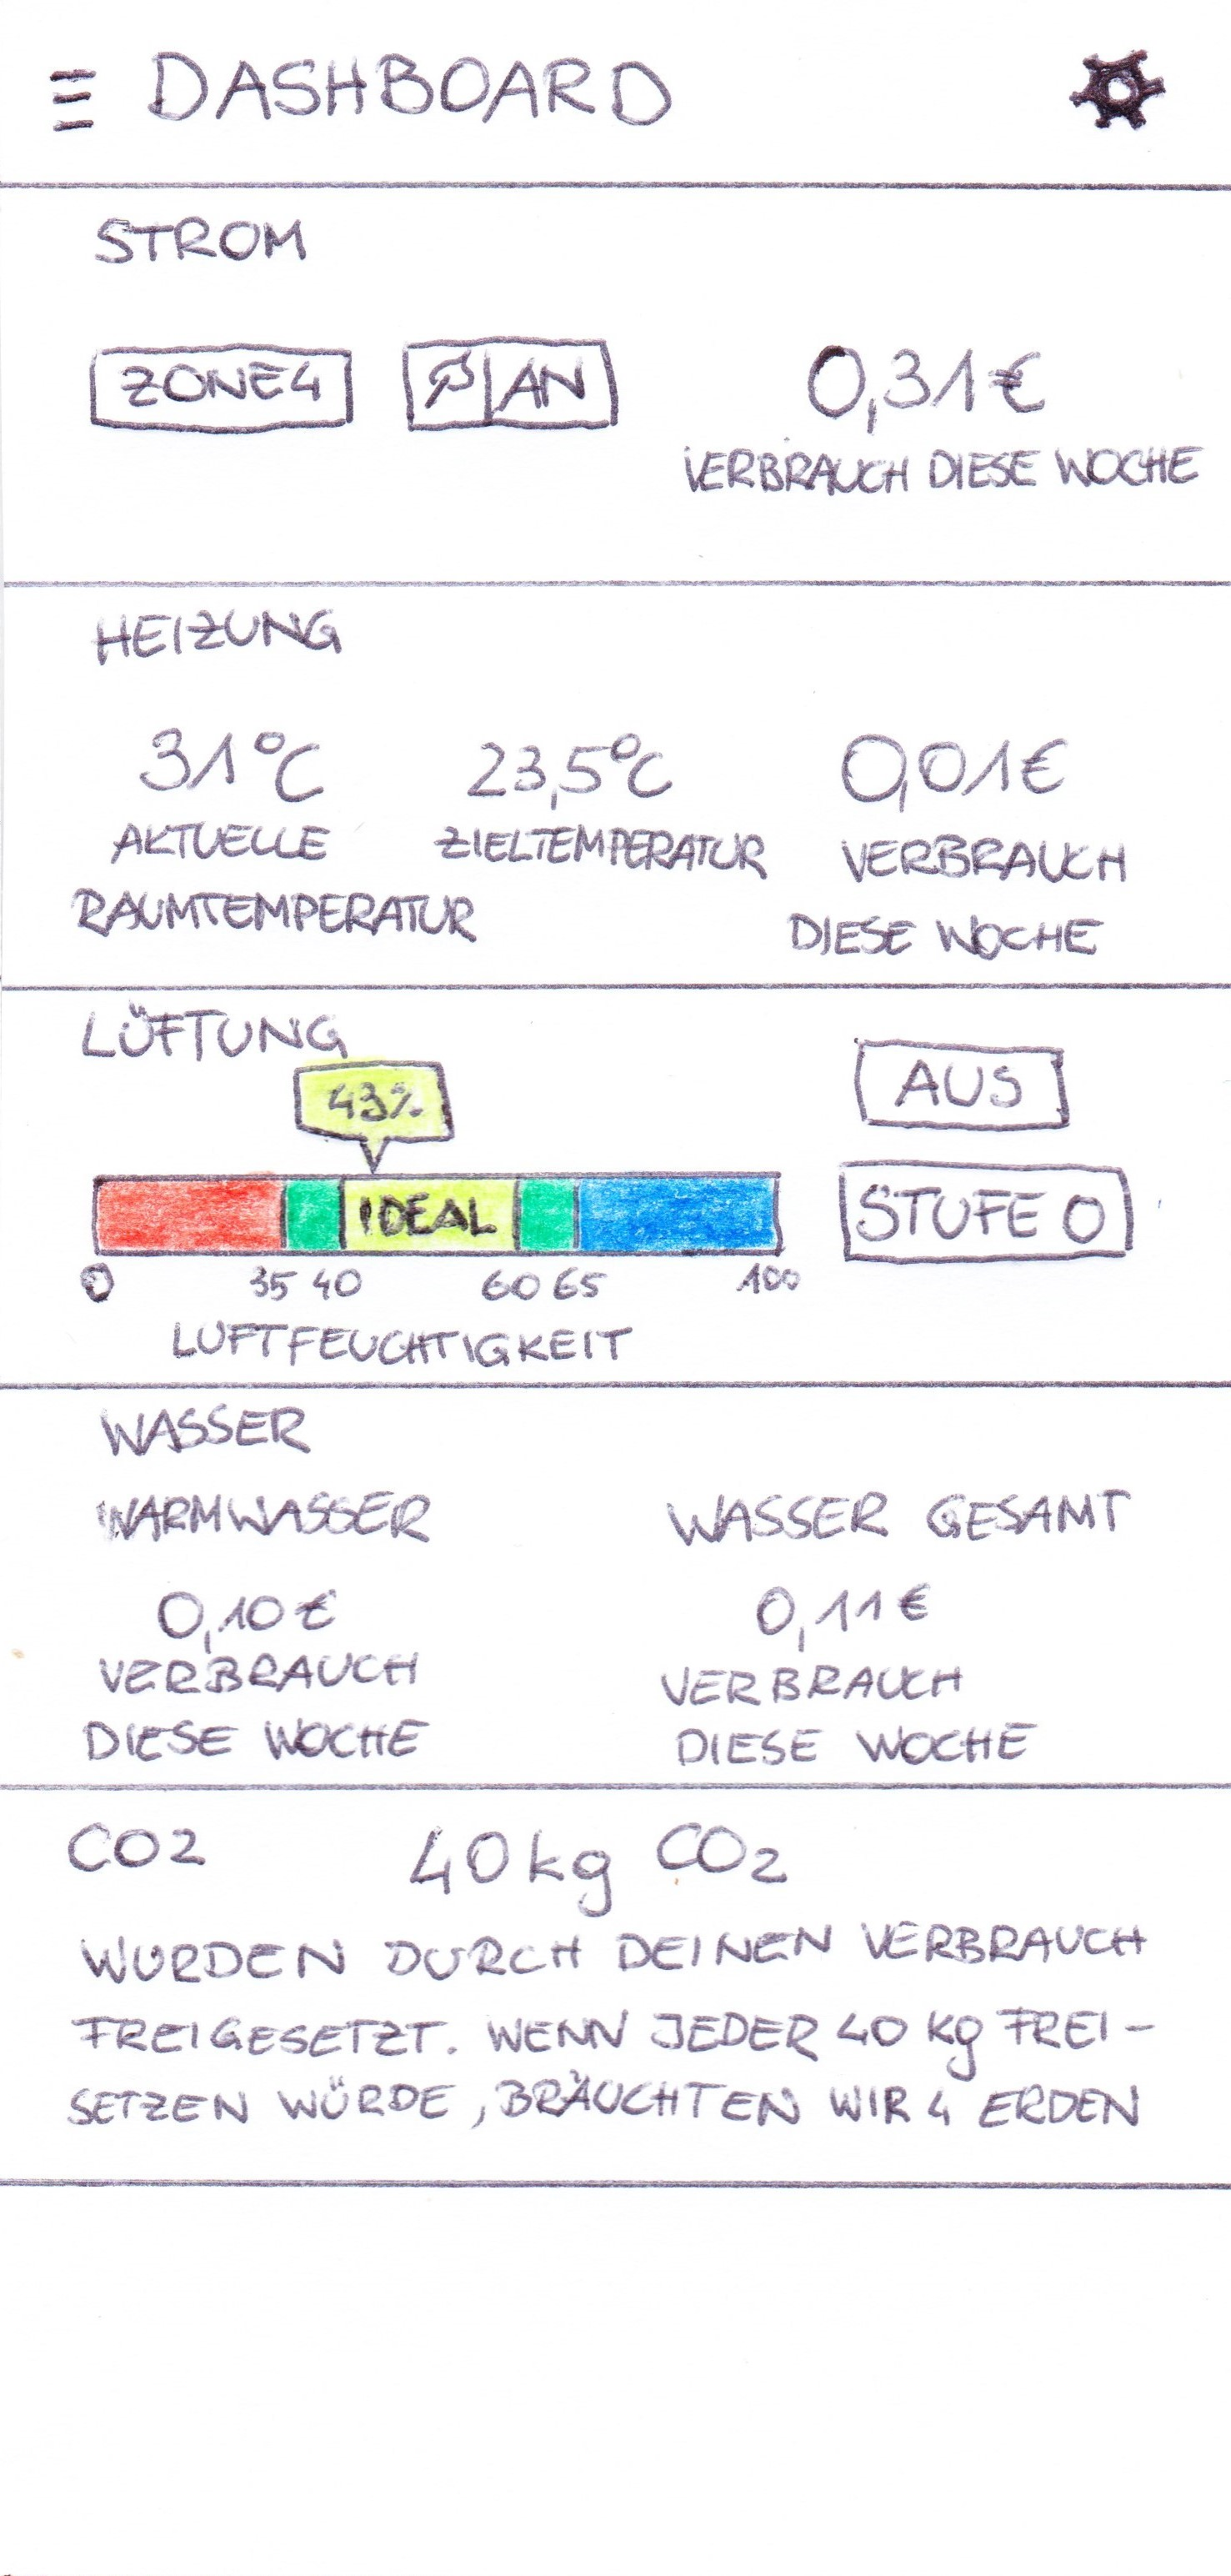
\includegraphics[width=\textwidth]{screens/dashboard_23}
		\subcaption{Optimizer and Indifferent}
		\label{fig:dashboard:optimizer}
	\end{subfigure}
	\caption{The proposed screen for the dashboard}
	\label{fig:dashboard} % \label has to be placed AFTER \caption (or \subcaption) to produce correct cross-references.
\end{figure}

\begin{figure}[h]
	\centering
	\begin{subfigure}[b]{0.24\columnwidth}
		\centering
		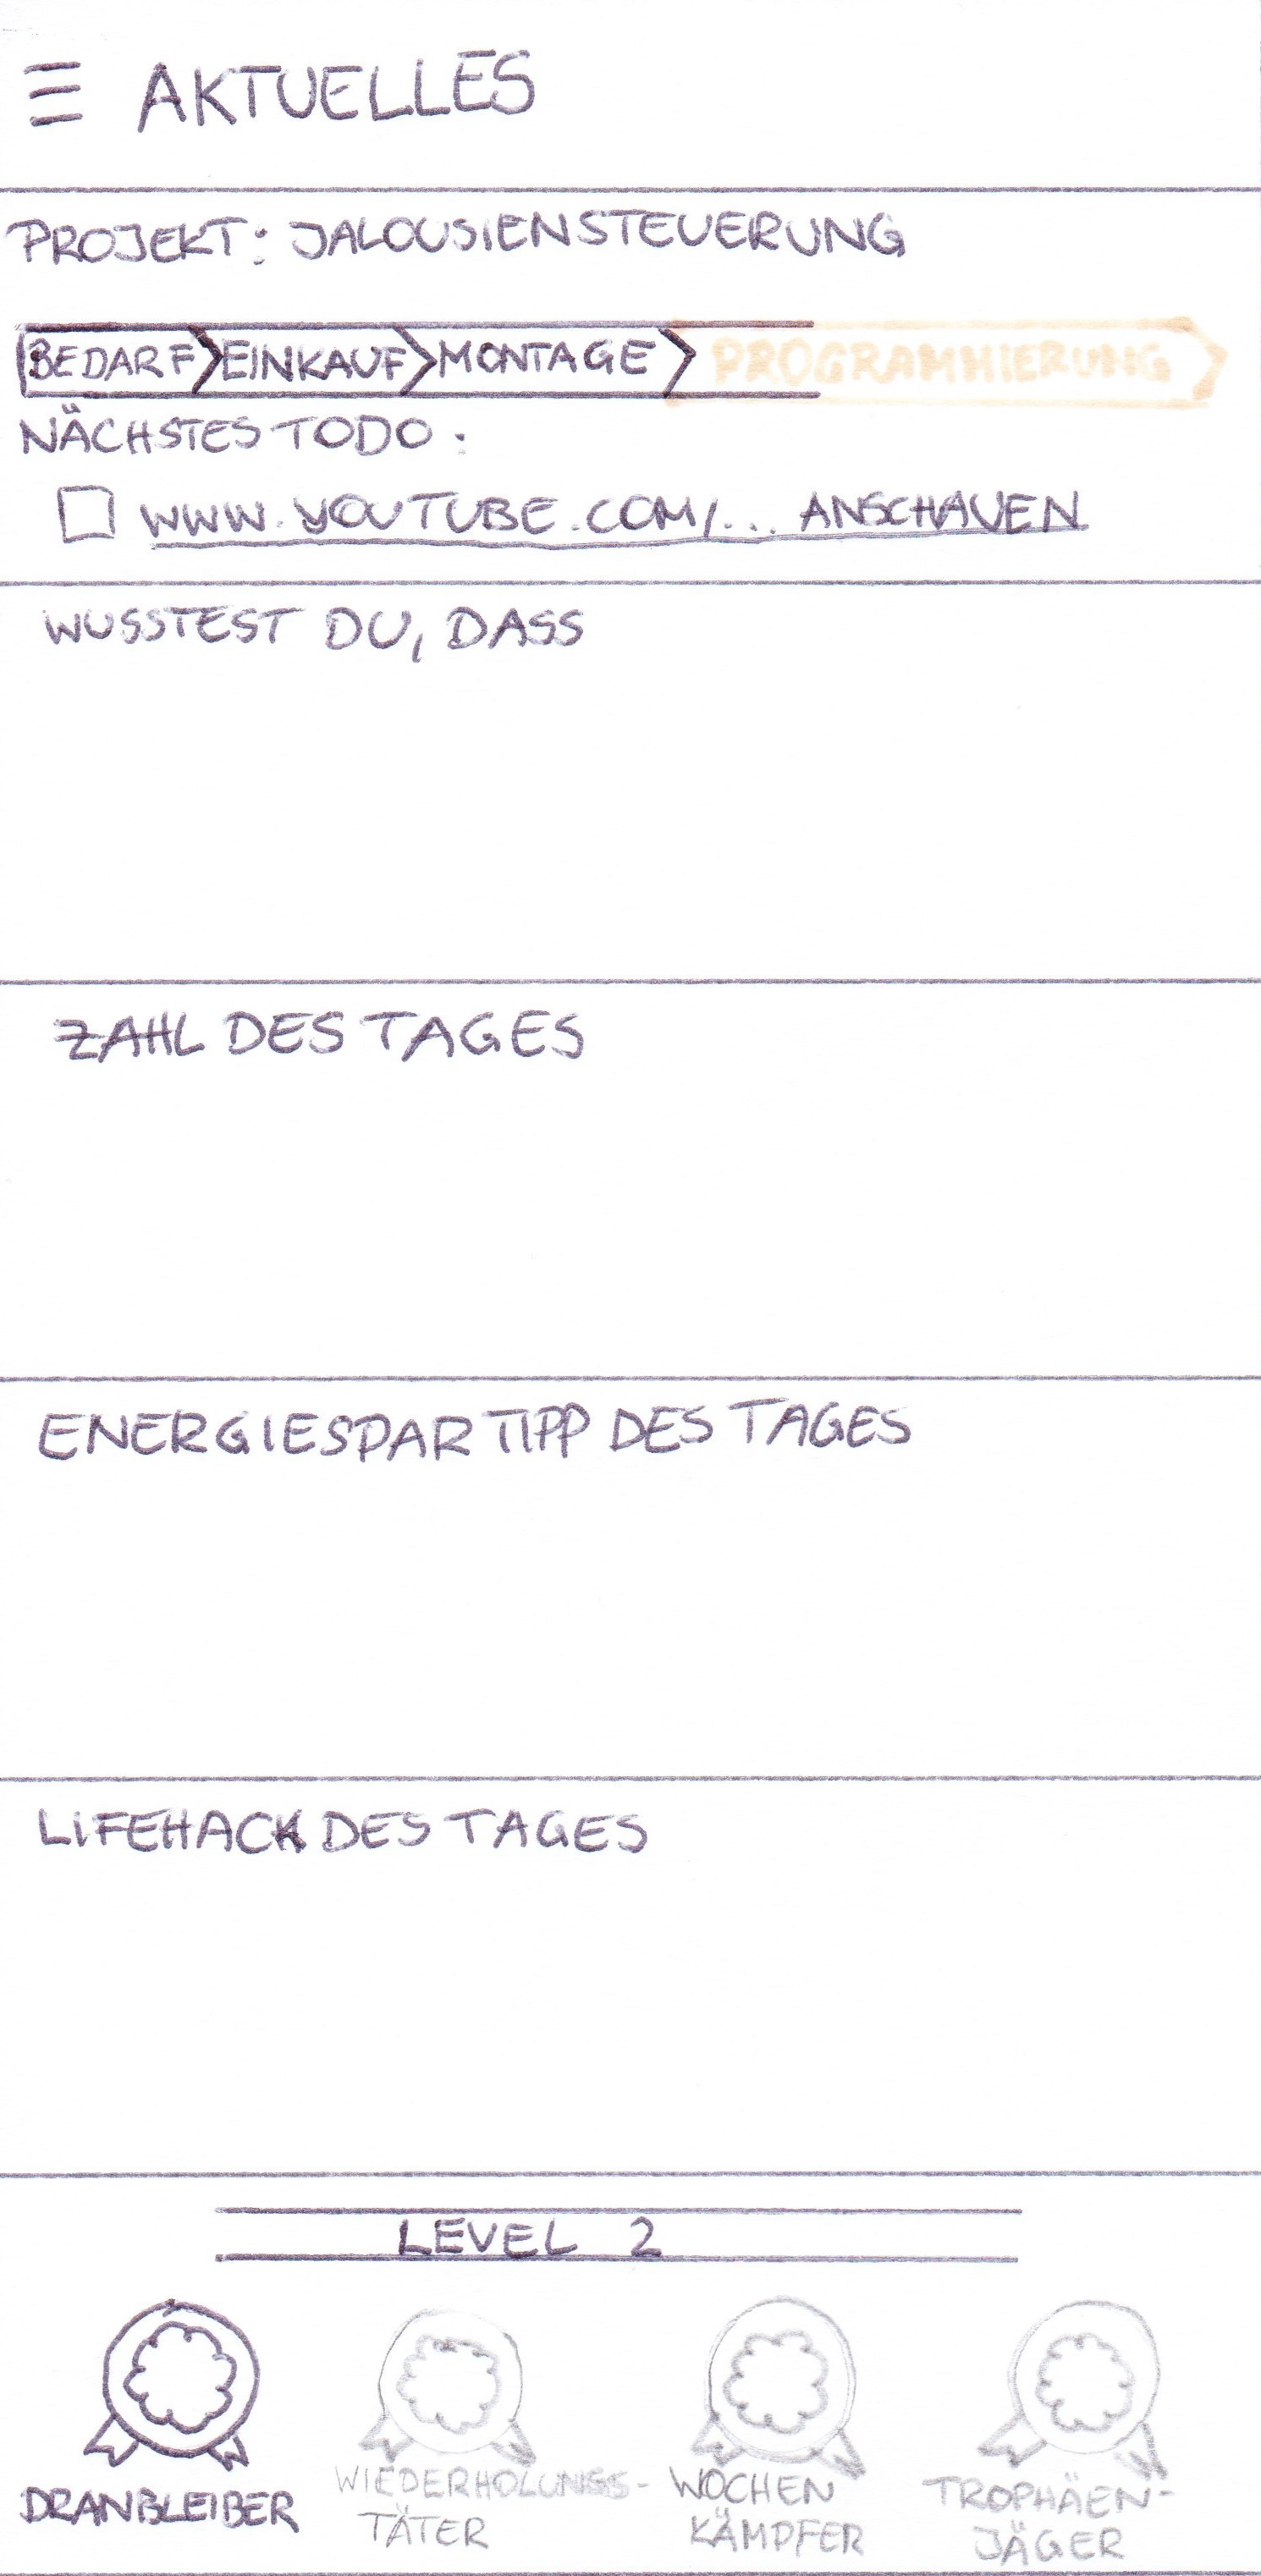
\includegraphics[width=\textwidth]{screens/aktuelles_14}
		\subcaption{Professional and Hedonist}
		\label{fig:aktuelles:professional}
	\end{subfigure}
	\begin{subfigure}[b]{0.24\columnwidth}
		\centering
		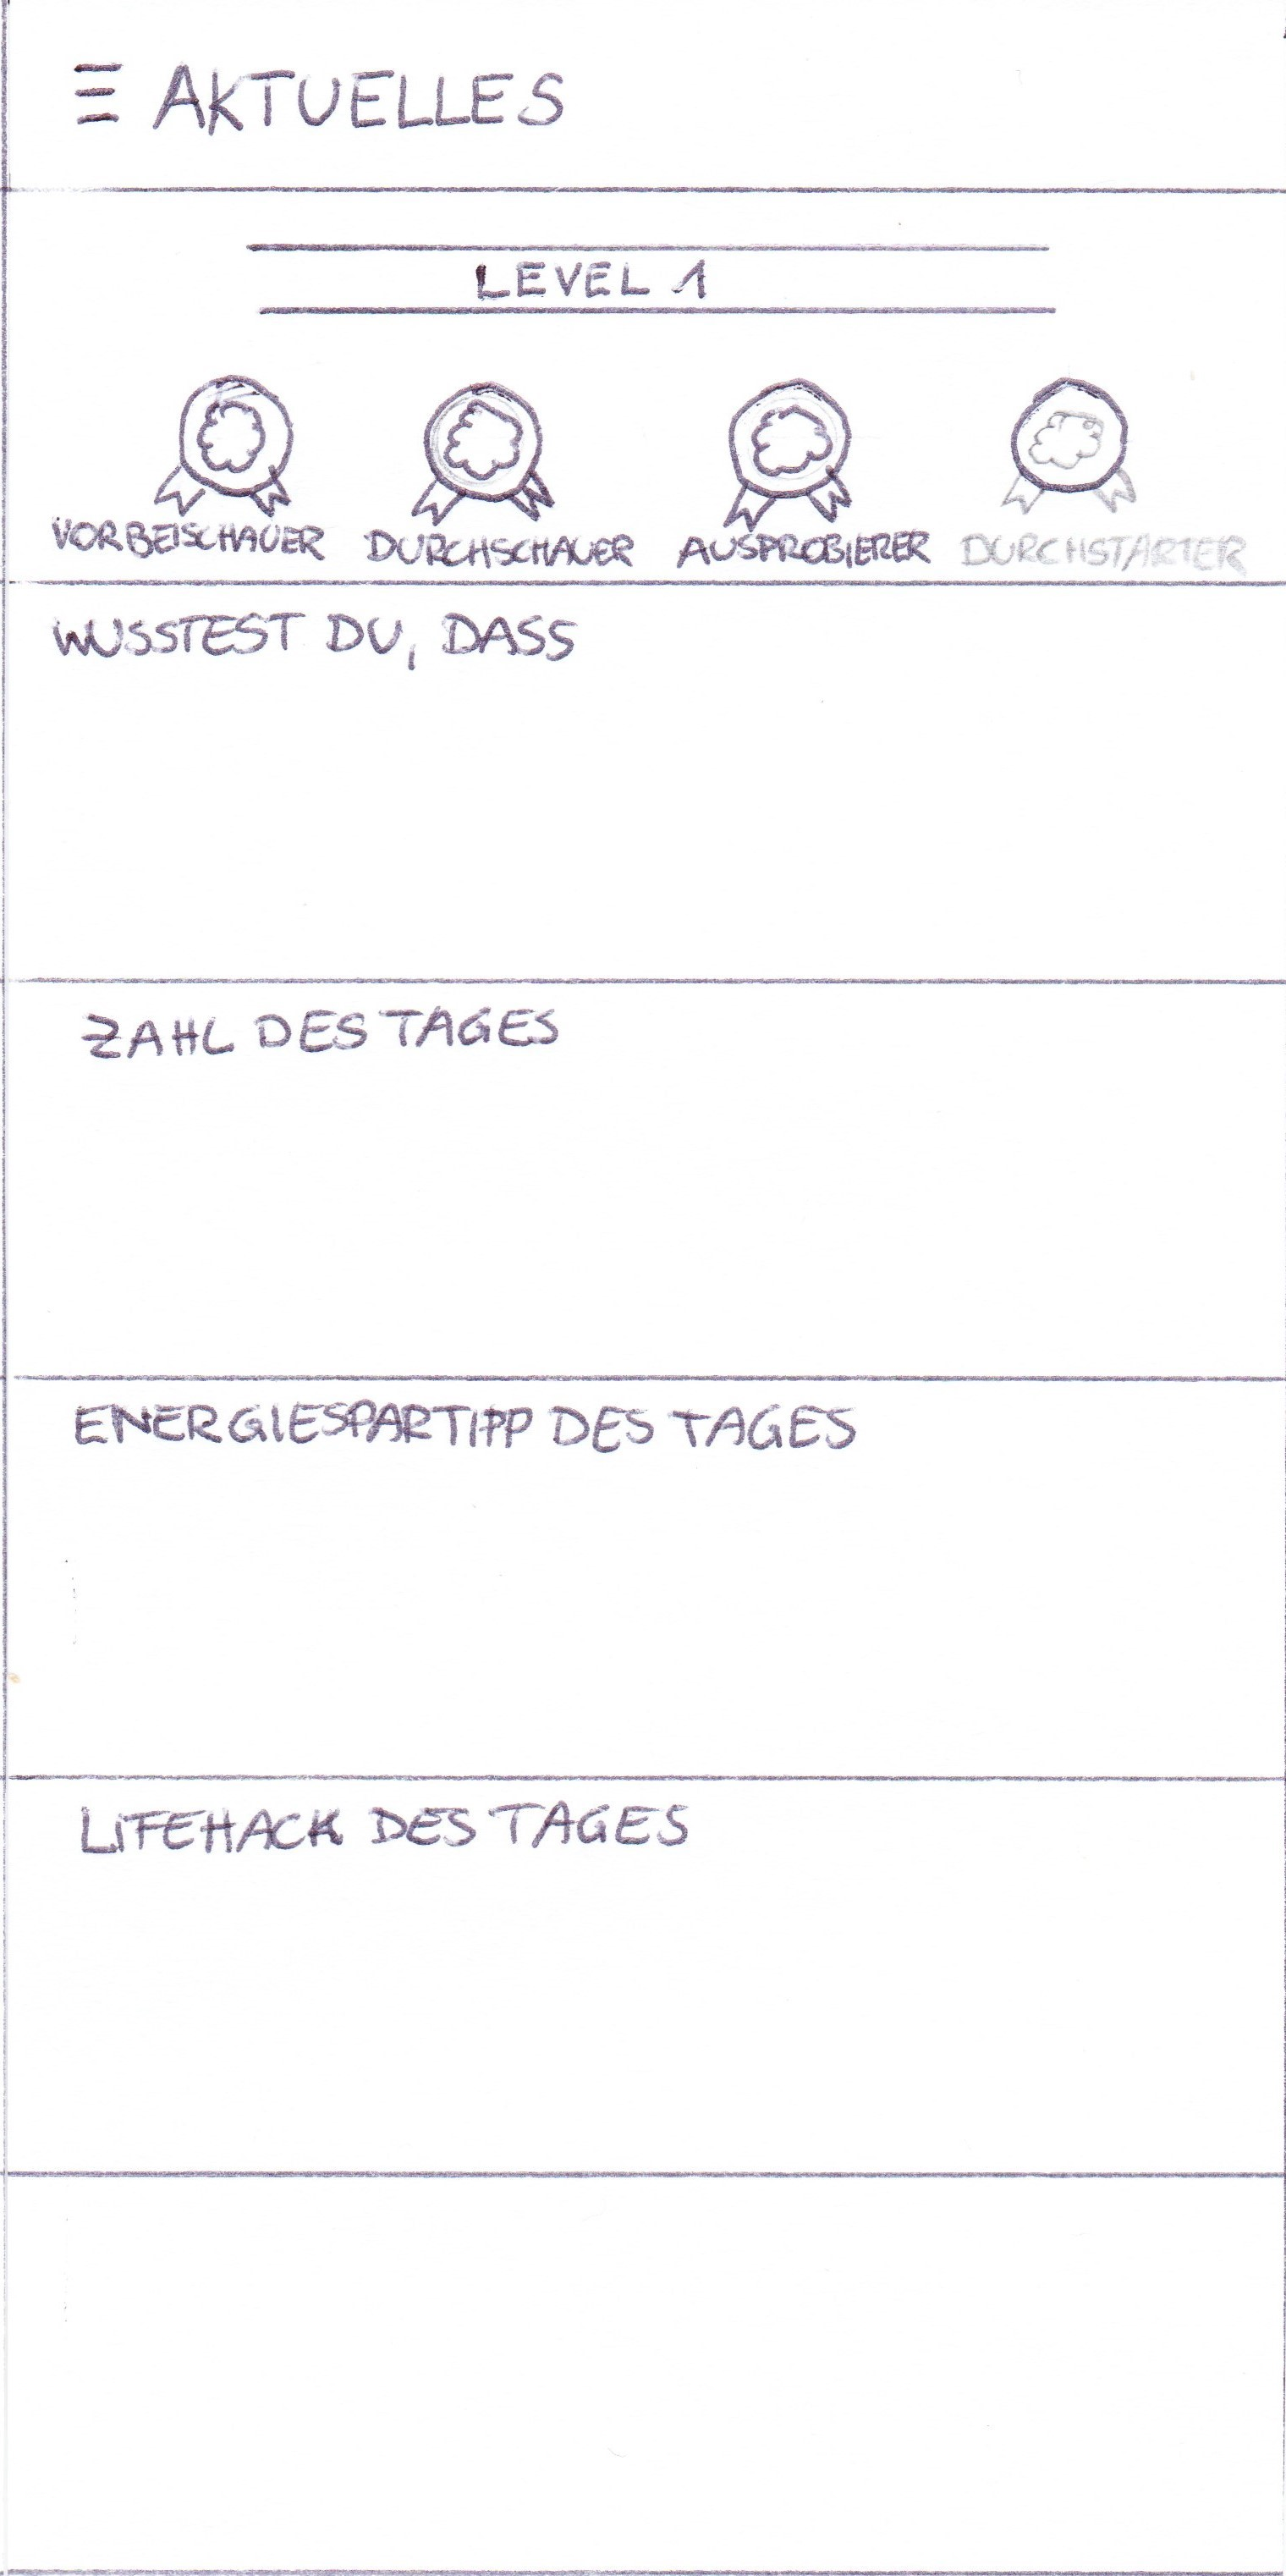
\includegraphics[width=\textwidth]{screens/aktuelles_23}
		\subcaption{Optimizer and Indifferent}
		\label{fig:aktuelles:optimizer}
	\end{subfigure}
	\caption{The proposed screen for the navigation drawer}
	\label{fig:aktuelles} % \label has to be placed AFTER \caption (or \subcaption) to produce correct cross-references.
\end{figure}

\begin{figure}[h]
	\centering
	\begin{subfigure}[b]{0.24\columnwidth}
		\centering
		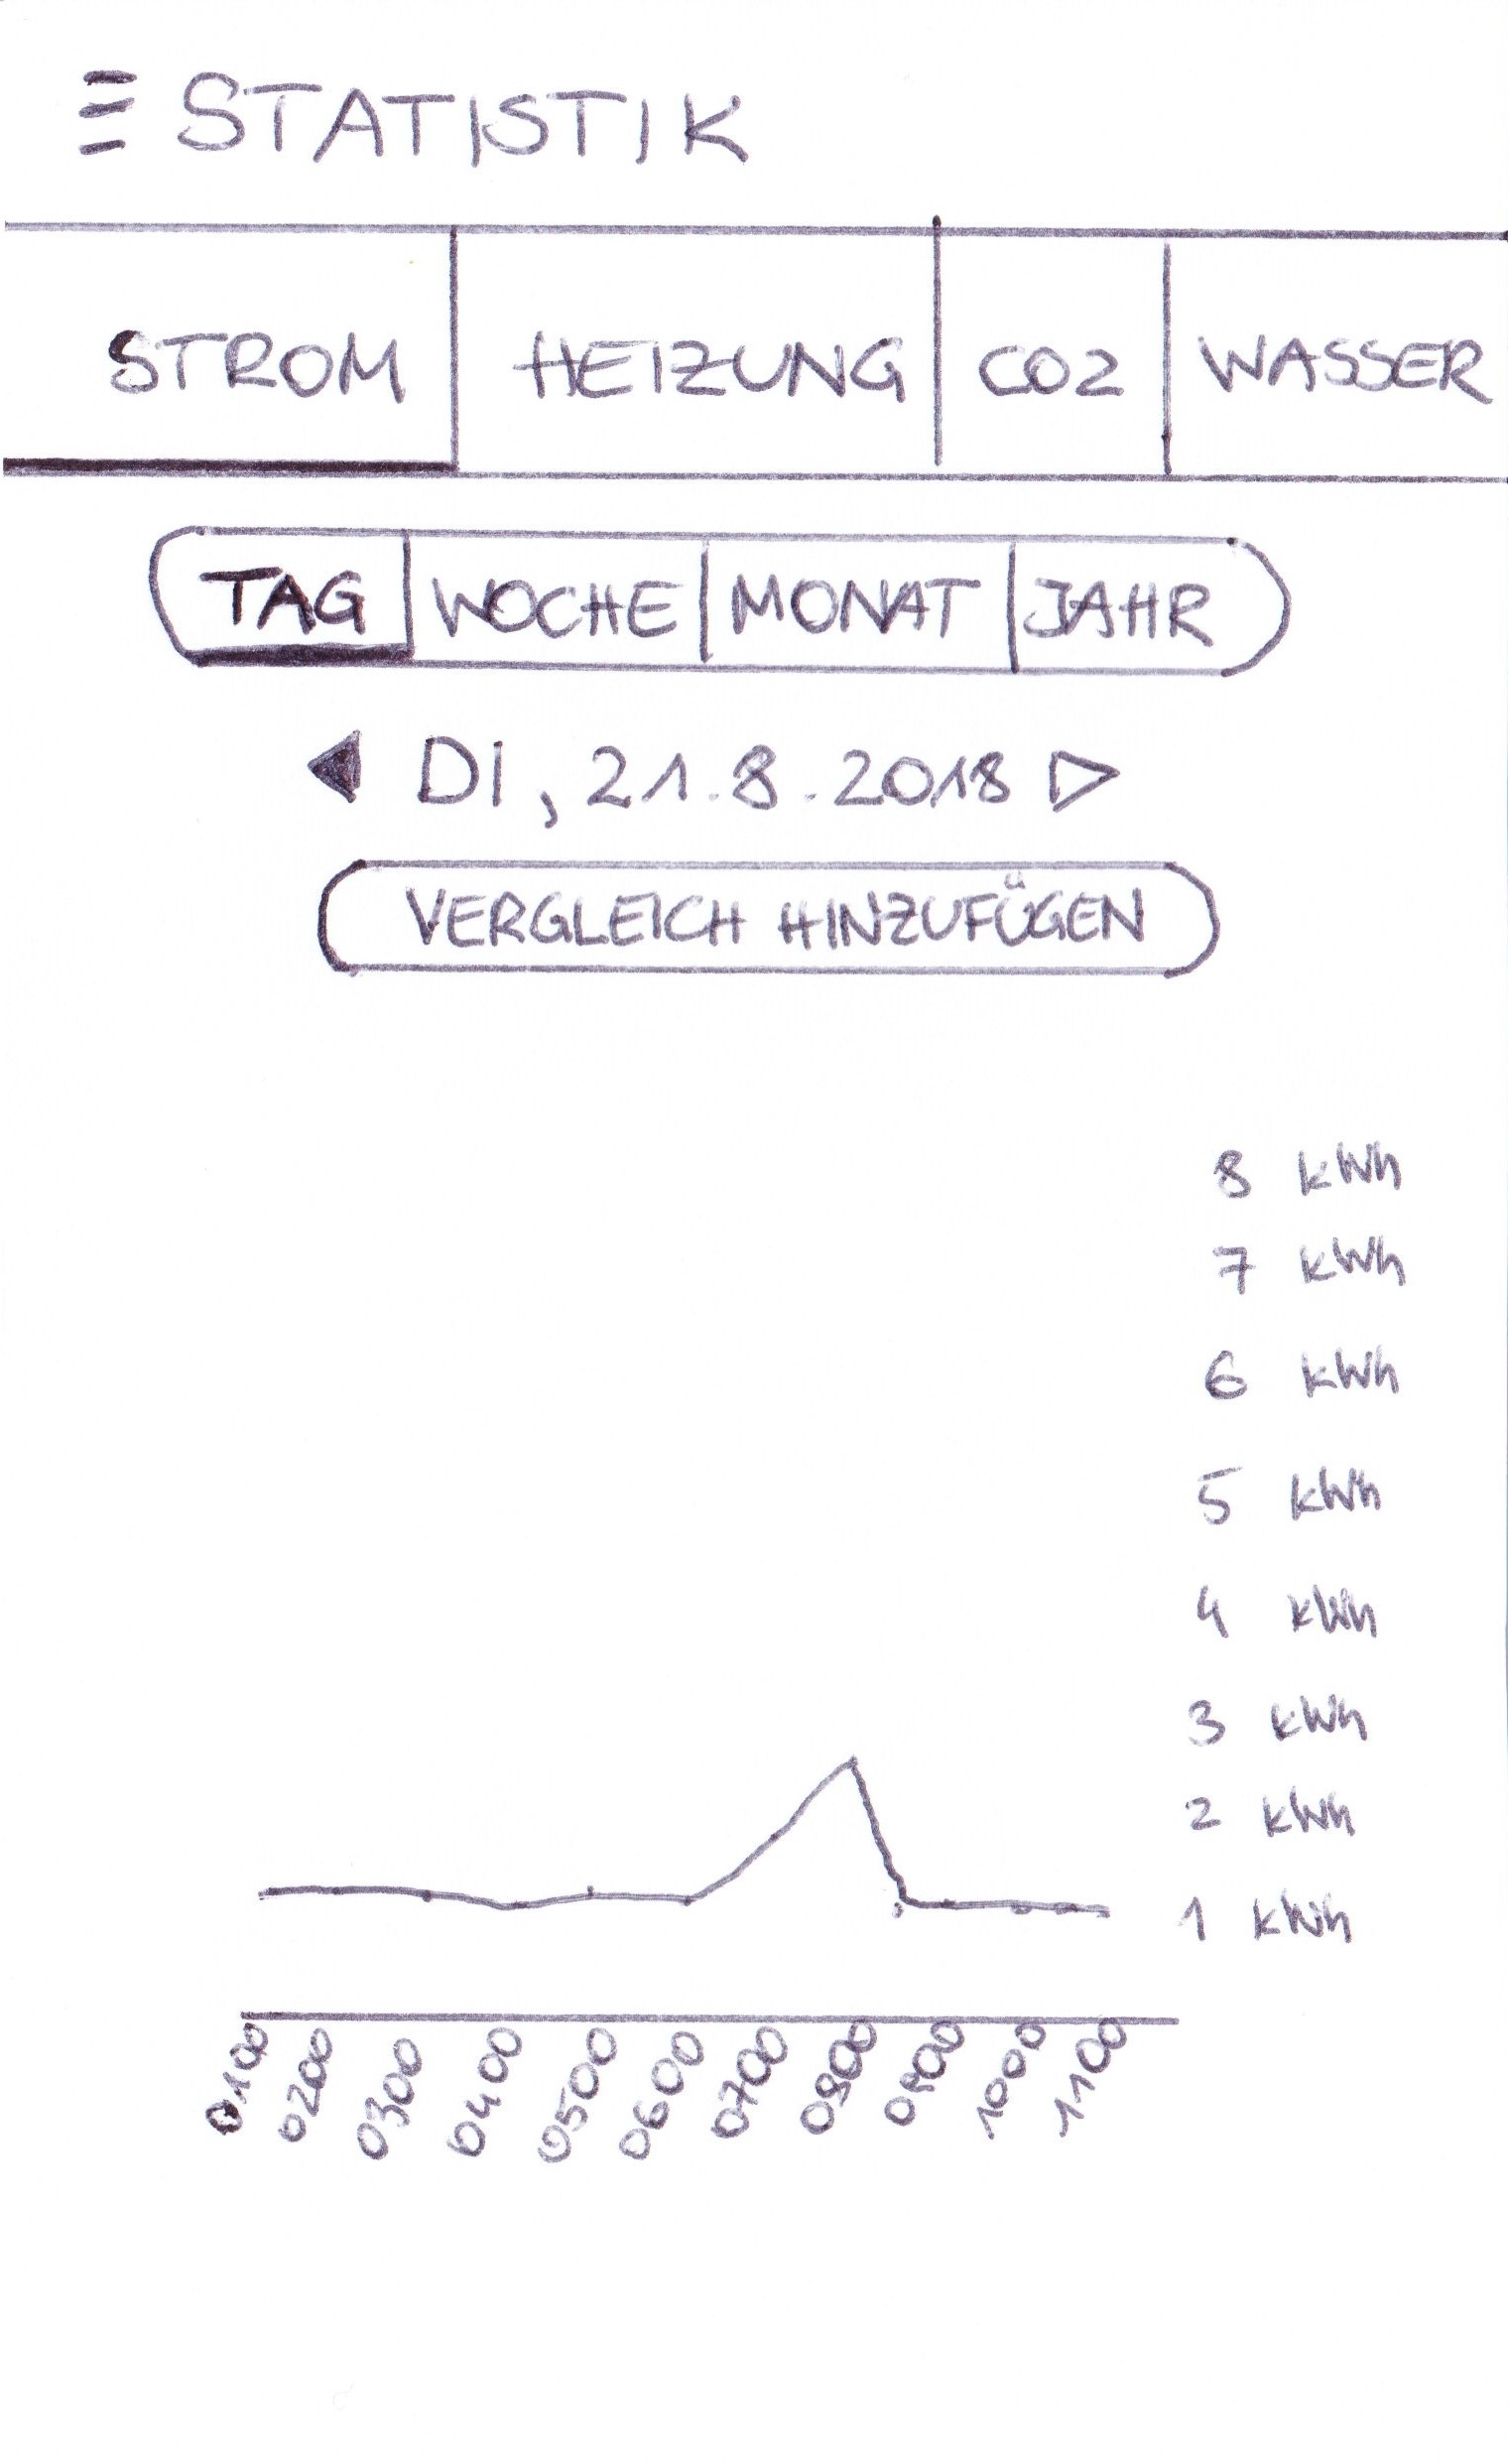
\includegraphics[width=\textwidth]{screens/Statistik_1234}
		\subcaption{Professional and Hedonist}
		\label{fig:statistik:professional}
	\end{subfigure}
	\begin{subfigure}[b]{0.24\columnwidth}
		\centering
		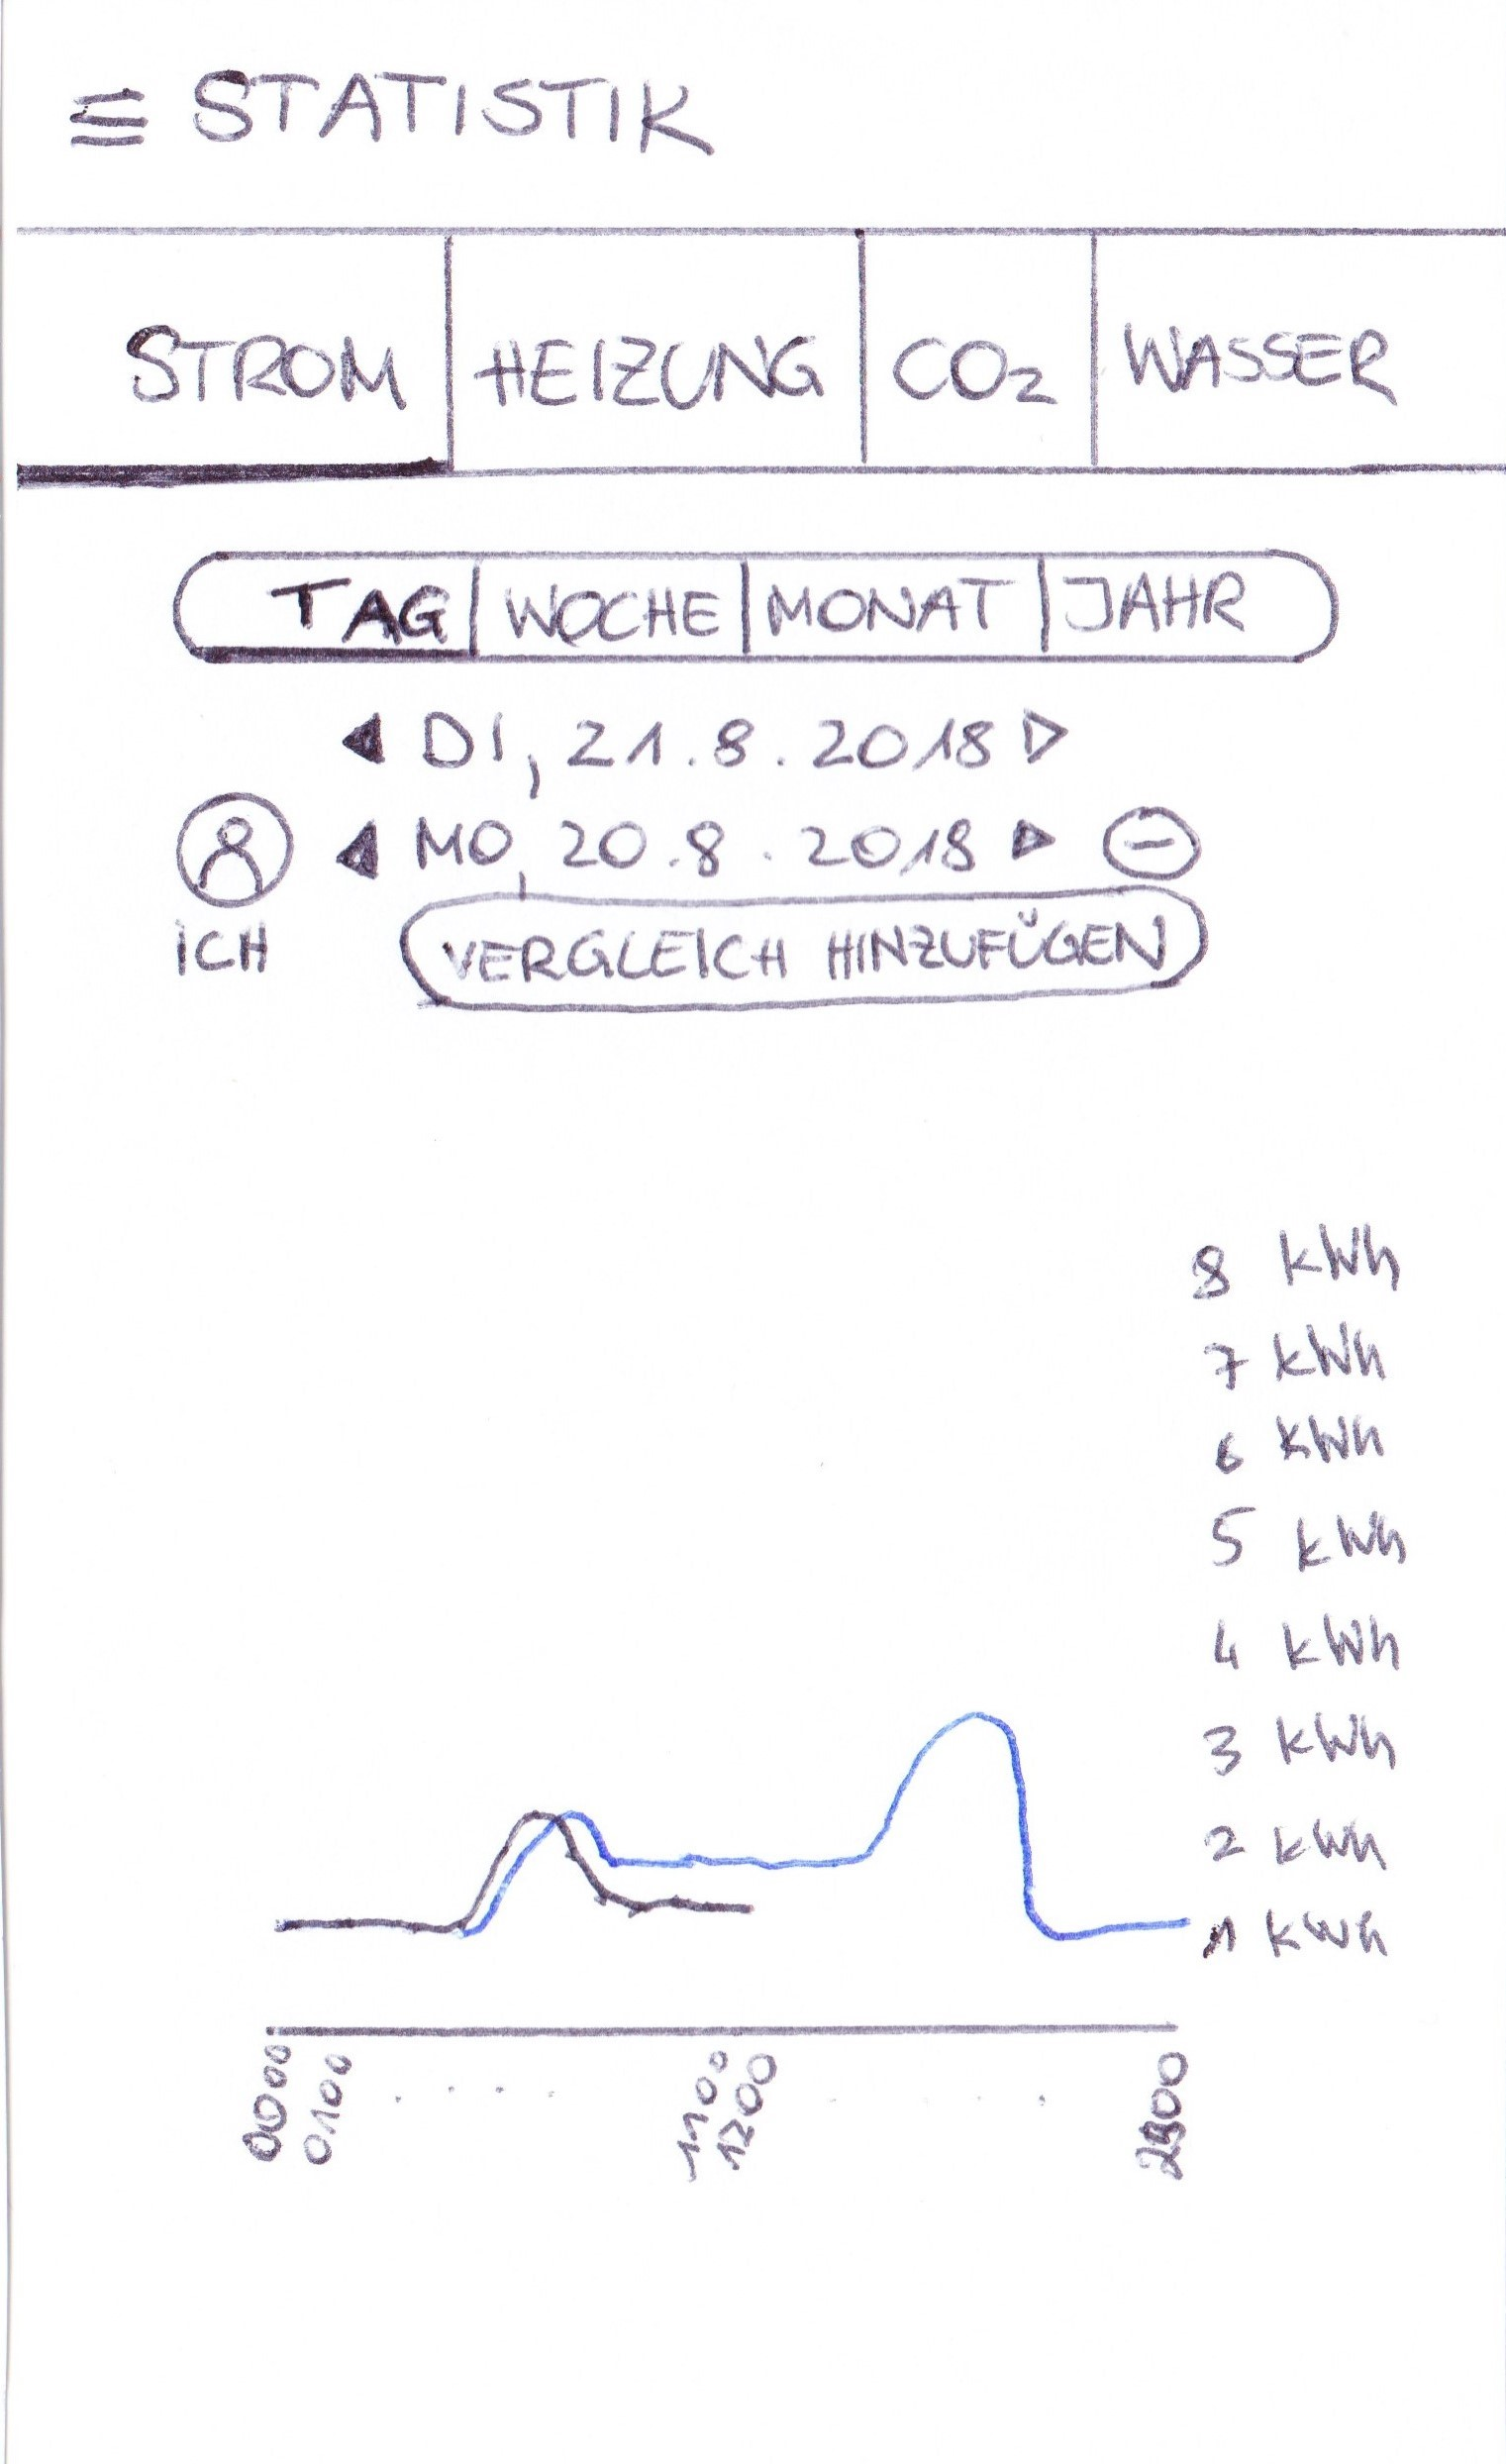
\includegraphics[width=\textwidth]{screens/Statistik_Vergleich}
		\subcaption{Optimizer and Indifferent}
		\label{fig:statistik:optimizer}
	\end{subfigure}
	\caption{The proposed screens for statistics}
	\label{fig:statistik} % \label has to be placed AFTER \caption (or \subcaption) to produce correct cross-references.
\end{figure}

\begin{figure}[h]
	\centering
	\begin{subfigure}[b]{0.24\columnwidth}
		\centering
		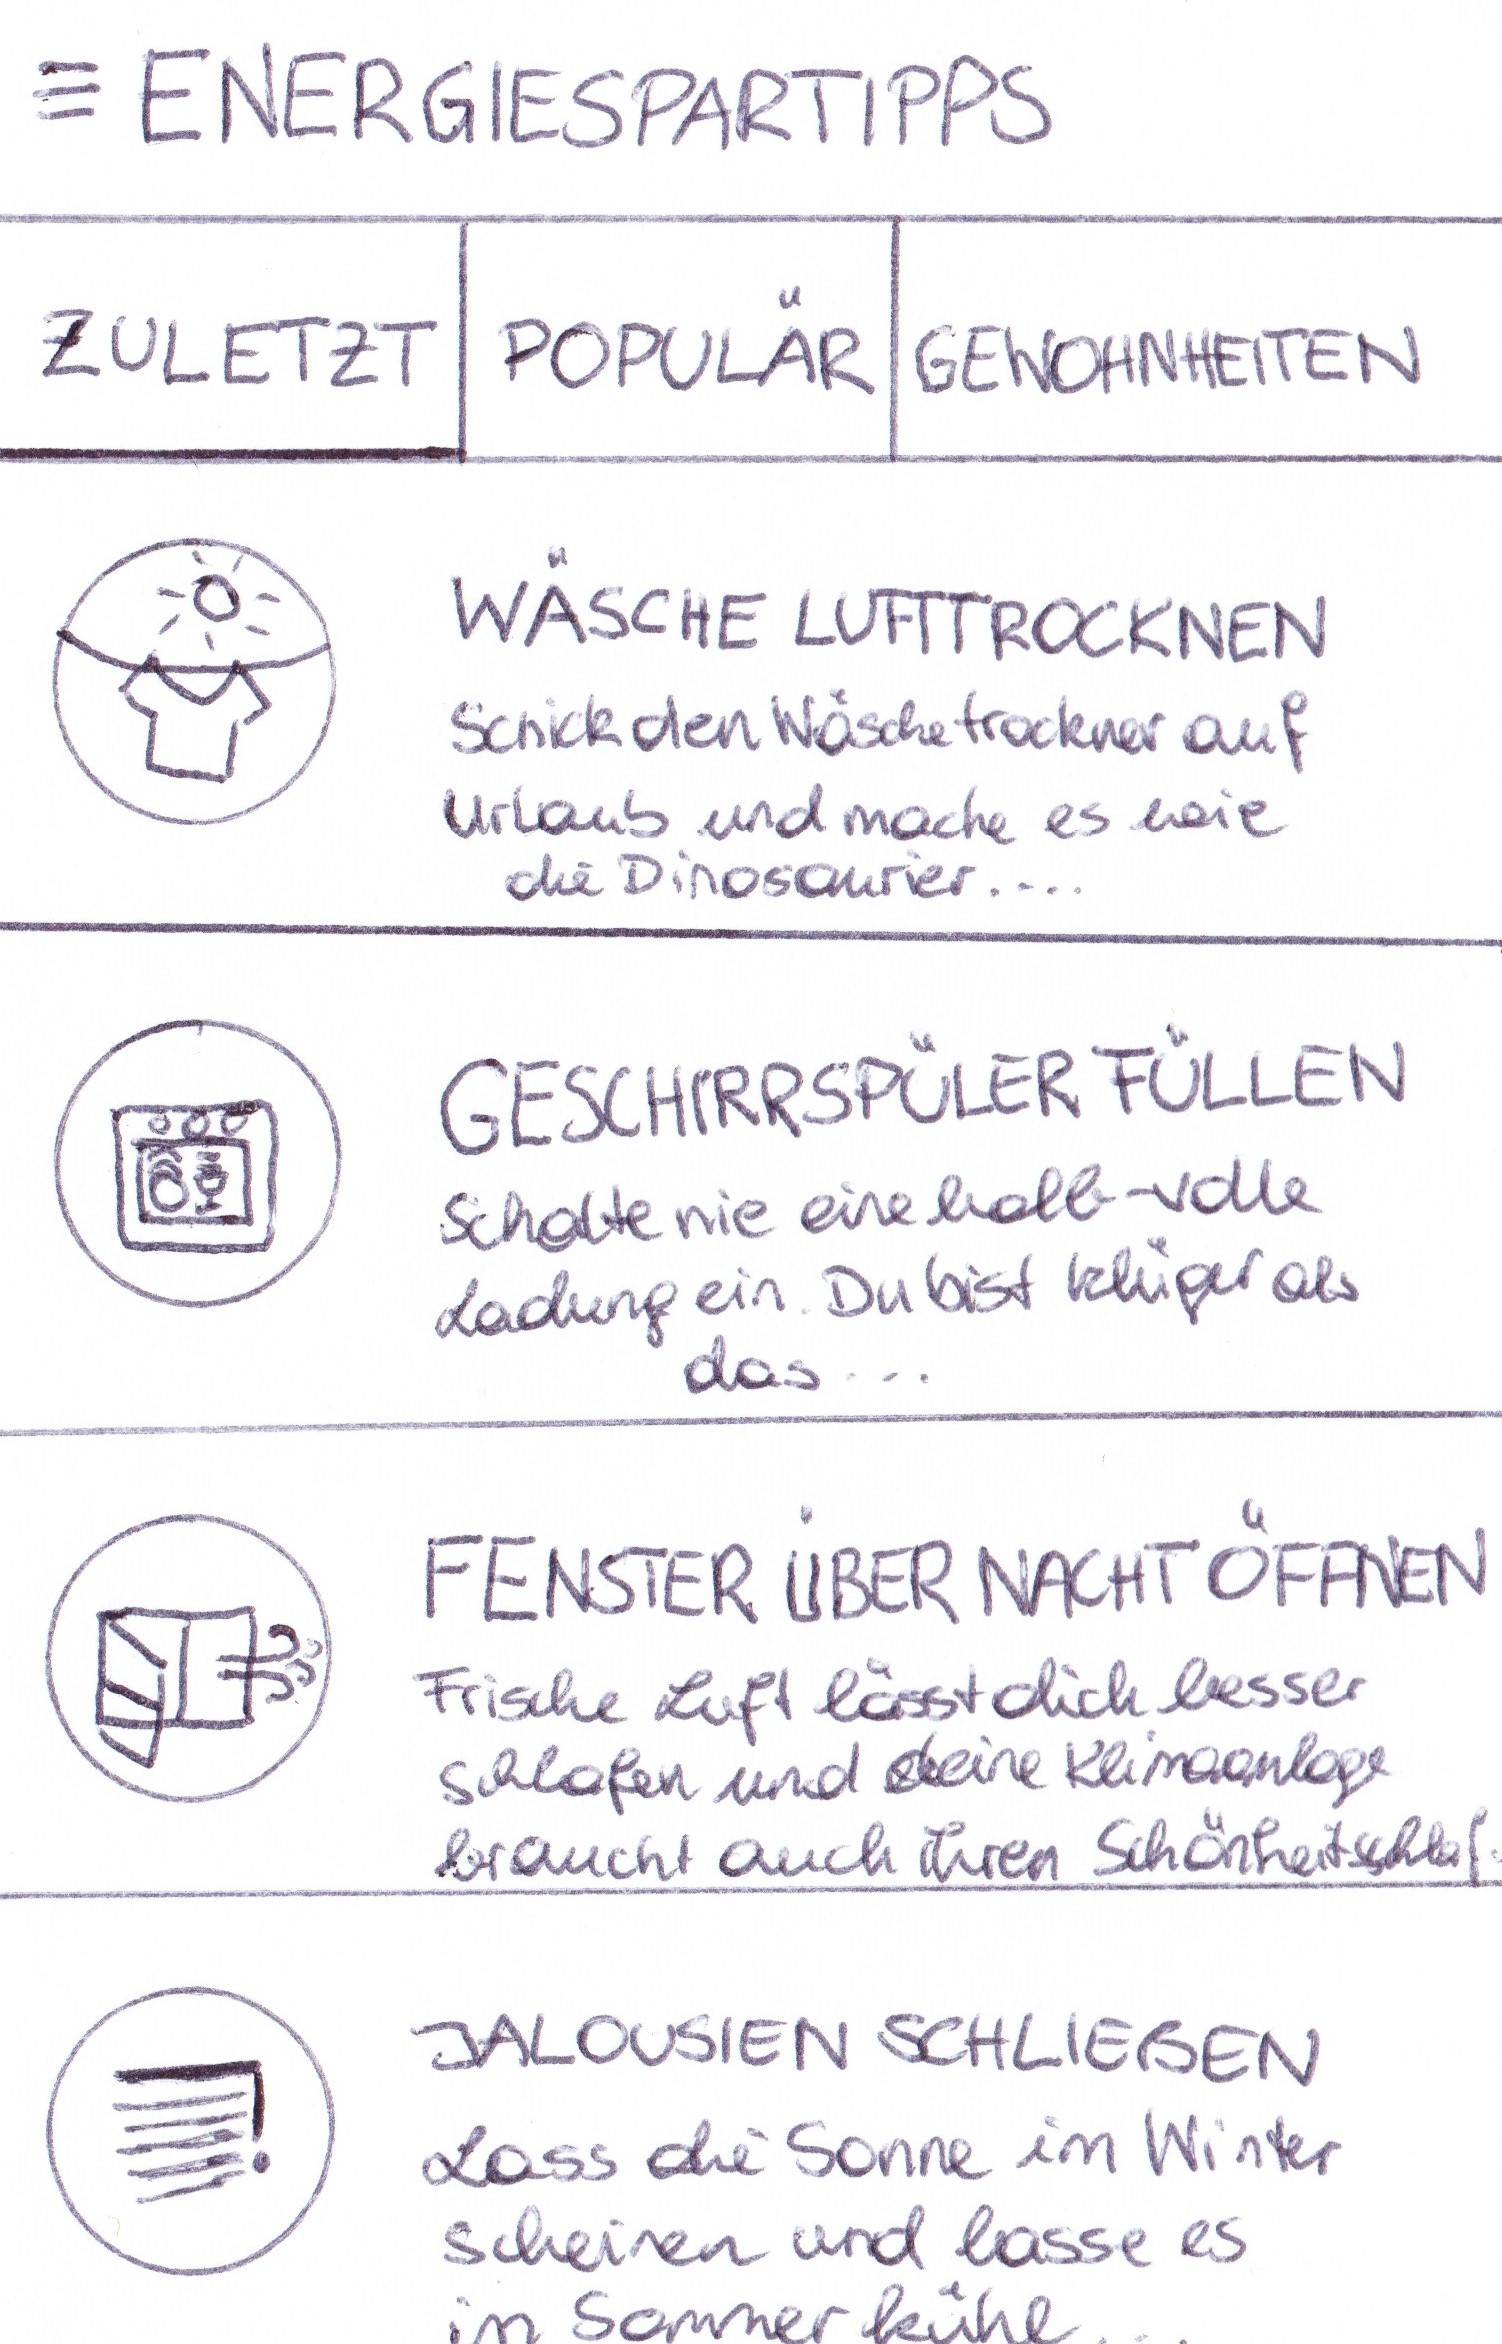
\includegraphics[width=\textwidth]{screens/tipp_1}
		\subcaption{Professional}
		\label{fig:tipps:professional}
	\end{subfigure}
	\begin{subfigure}[b]{0.24\columnwidth}
		\centering
		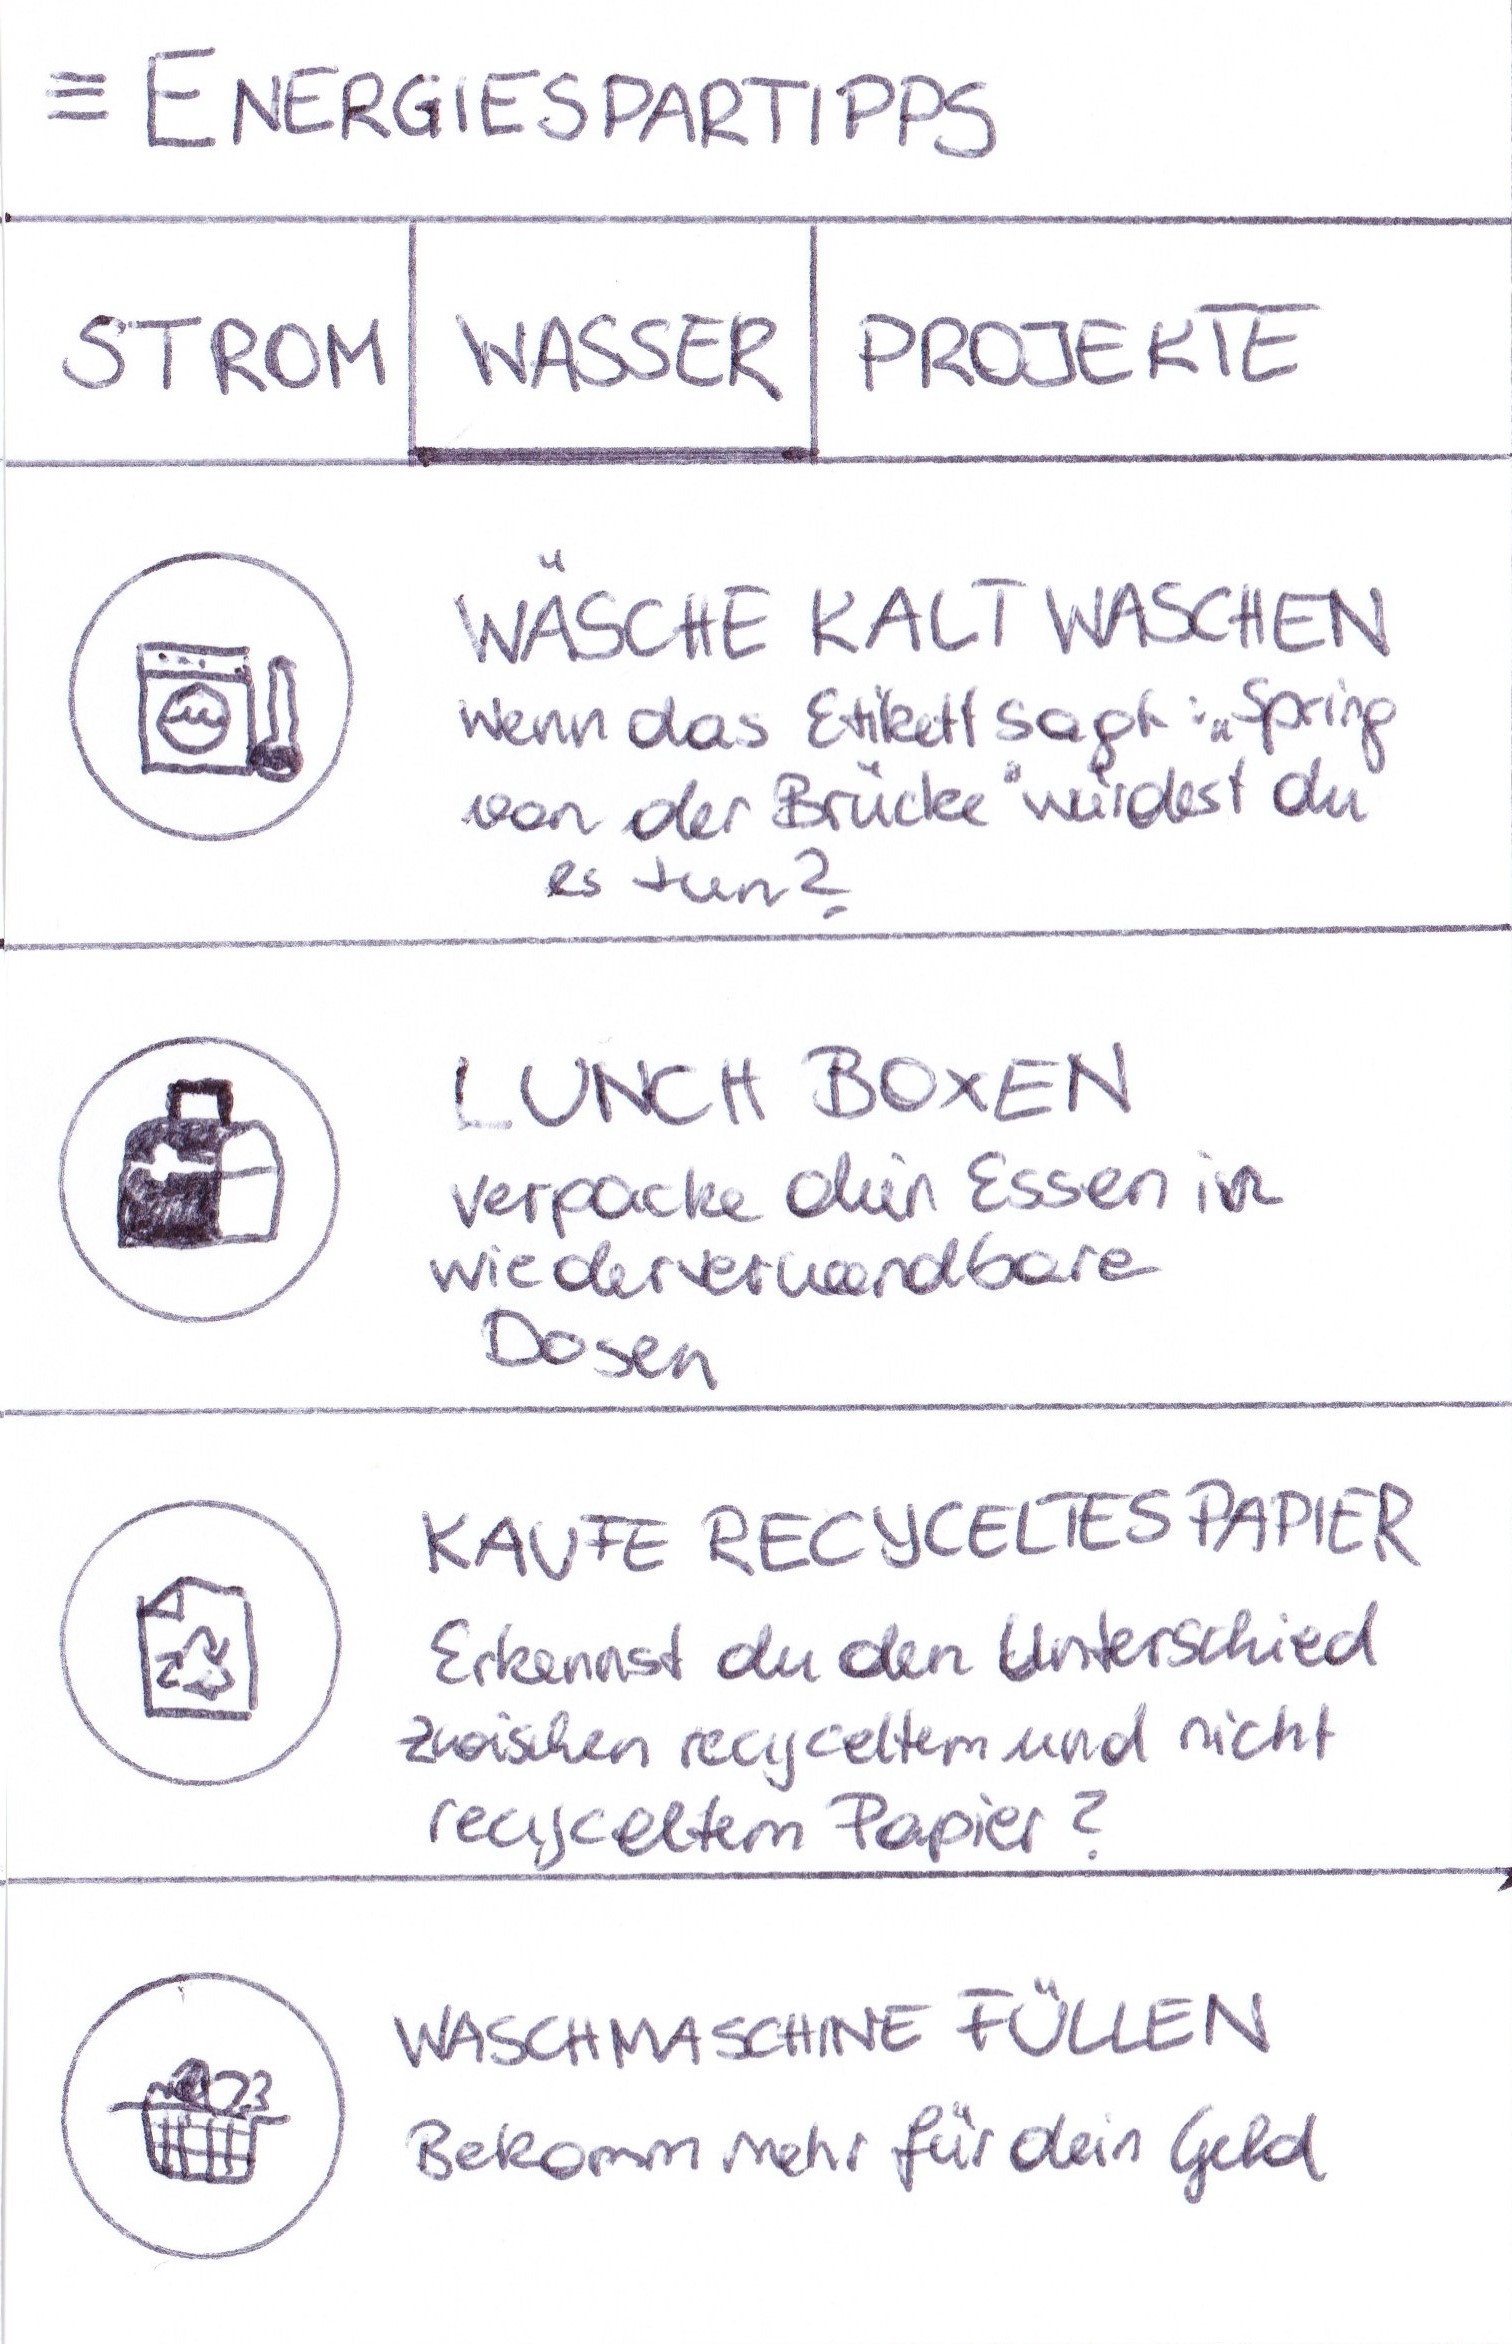
\includegraphics[width=\textwidth]{screens/tipp_2}
		\subcaption{Optimizer}
		\label{fig:tipps:optimizer}
	\end{subfigure}
	\begin{subfigure}[b]{0.24\columnwidth}
		\centering
		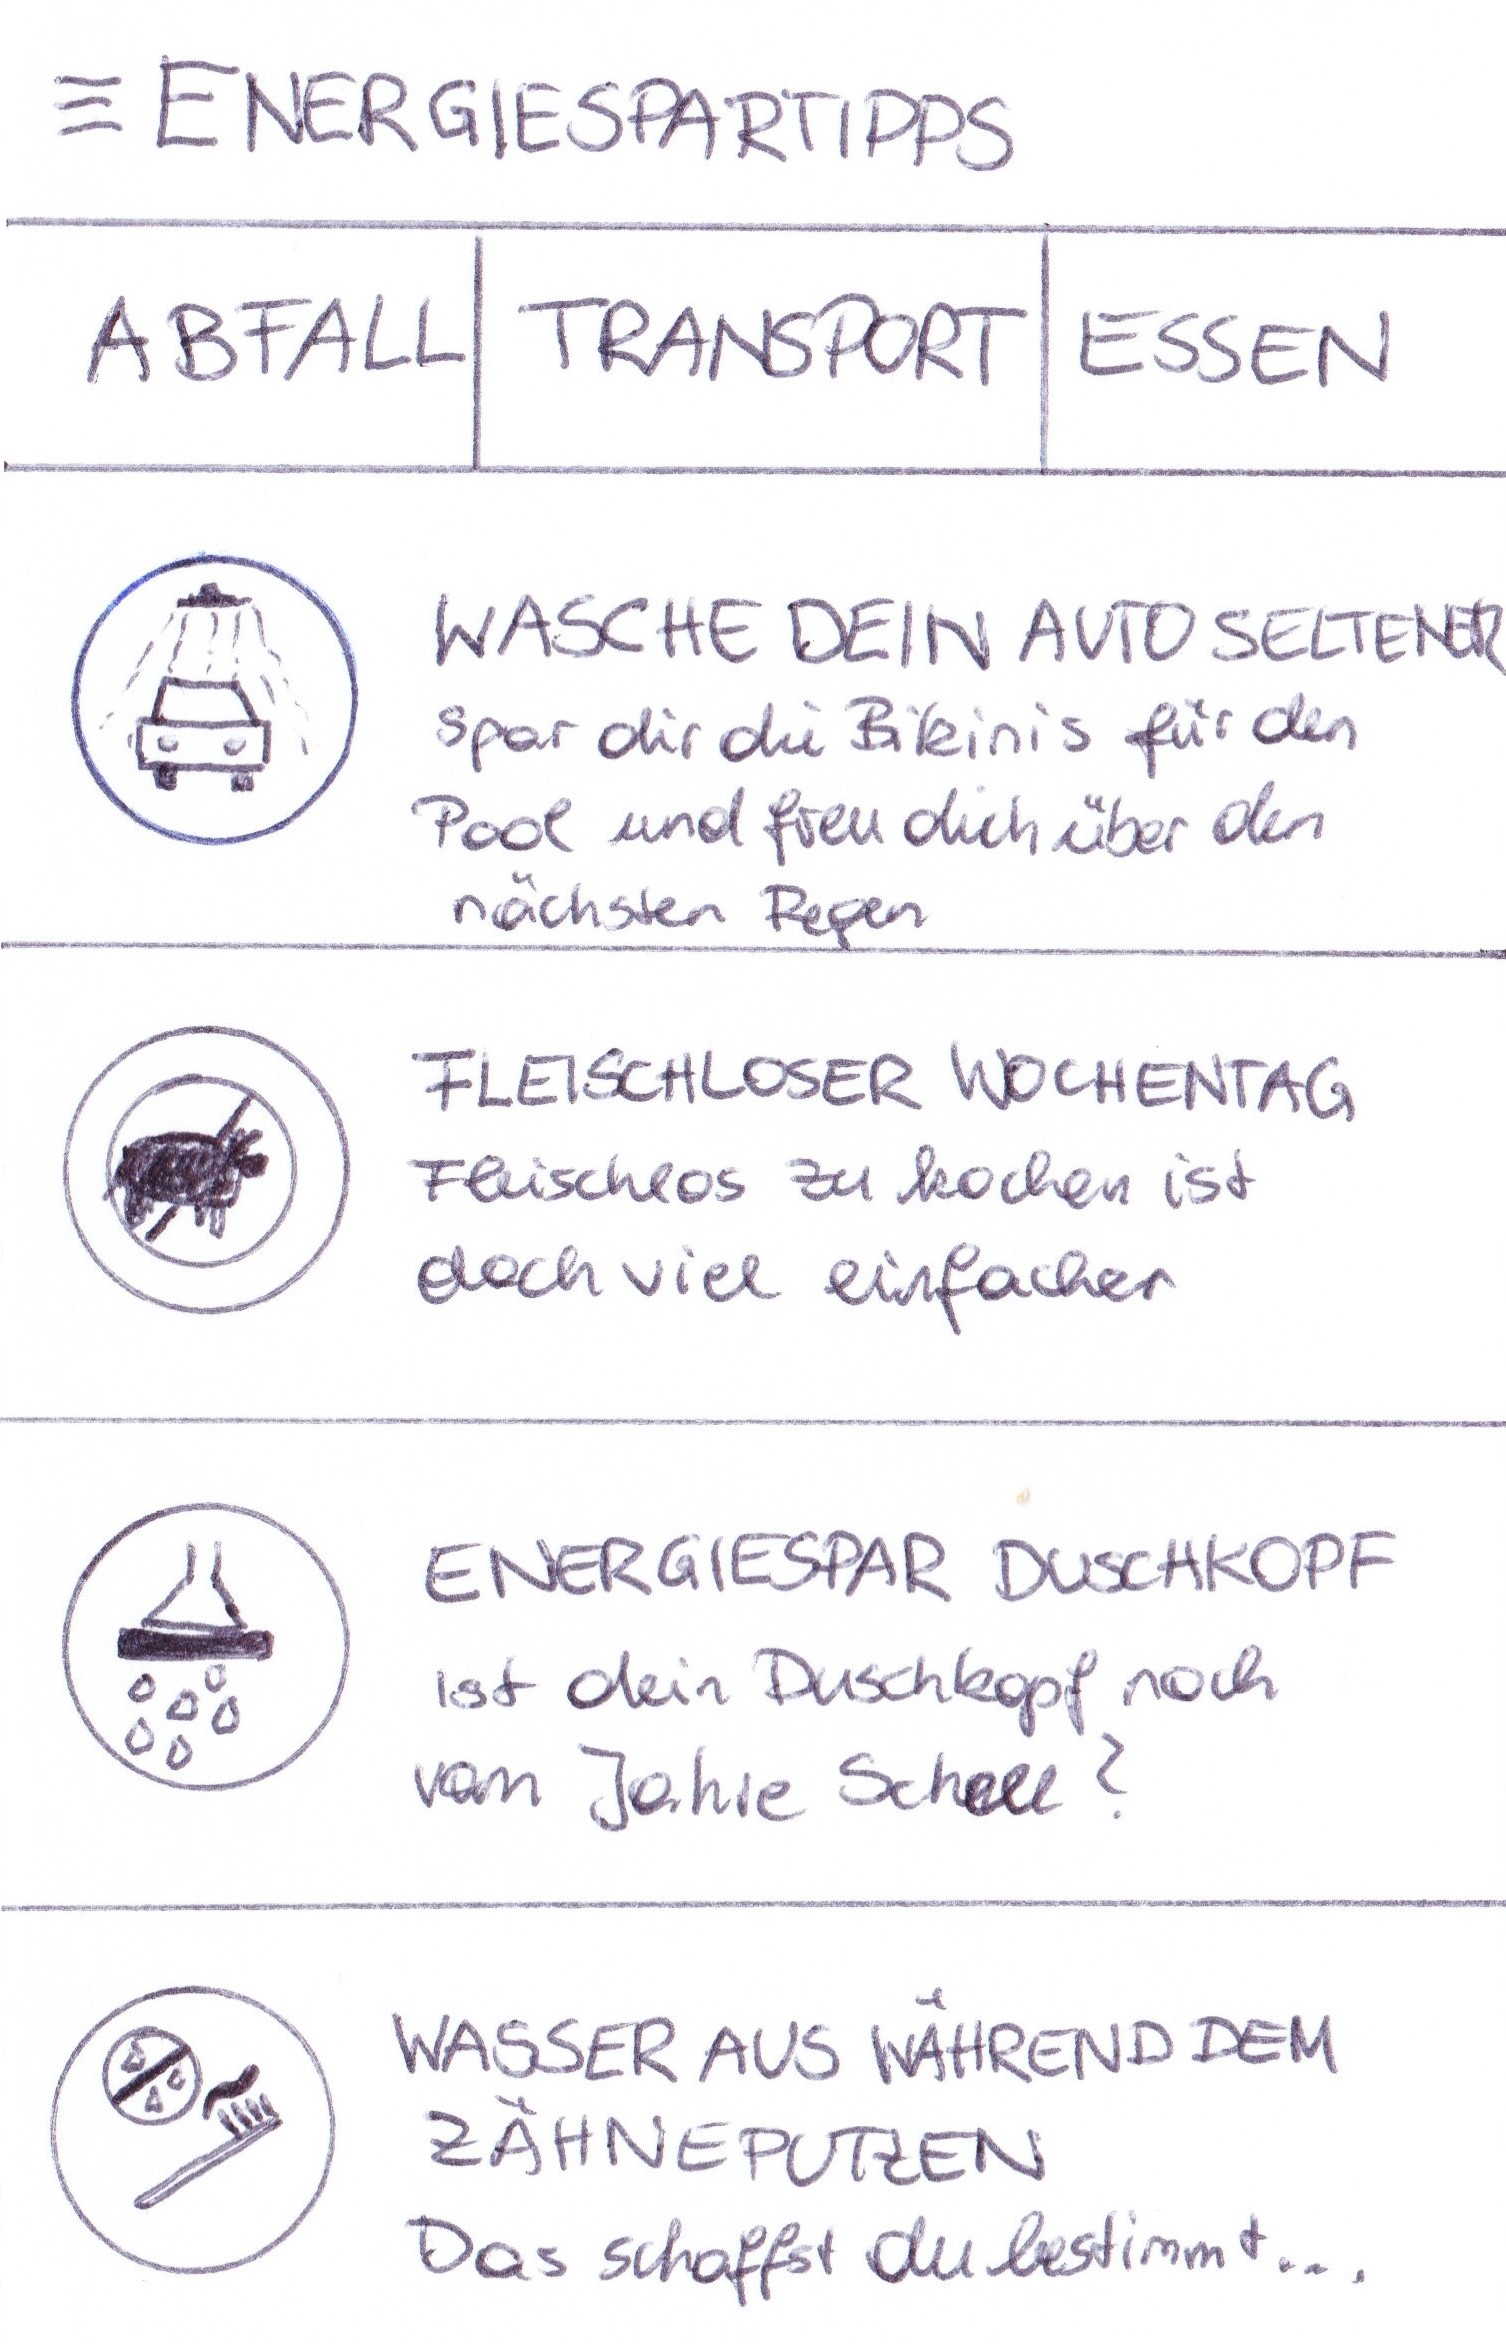
\includegraphics[width=\textwidth]{screens/tipp_3}
		\subcaption{Indifferent}
		\label{fig:tipps:indifferent}
	\end{subfigure}
	\begin{subfigure}[b]{0.24\columnwidth}
		\centering
		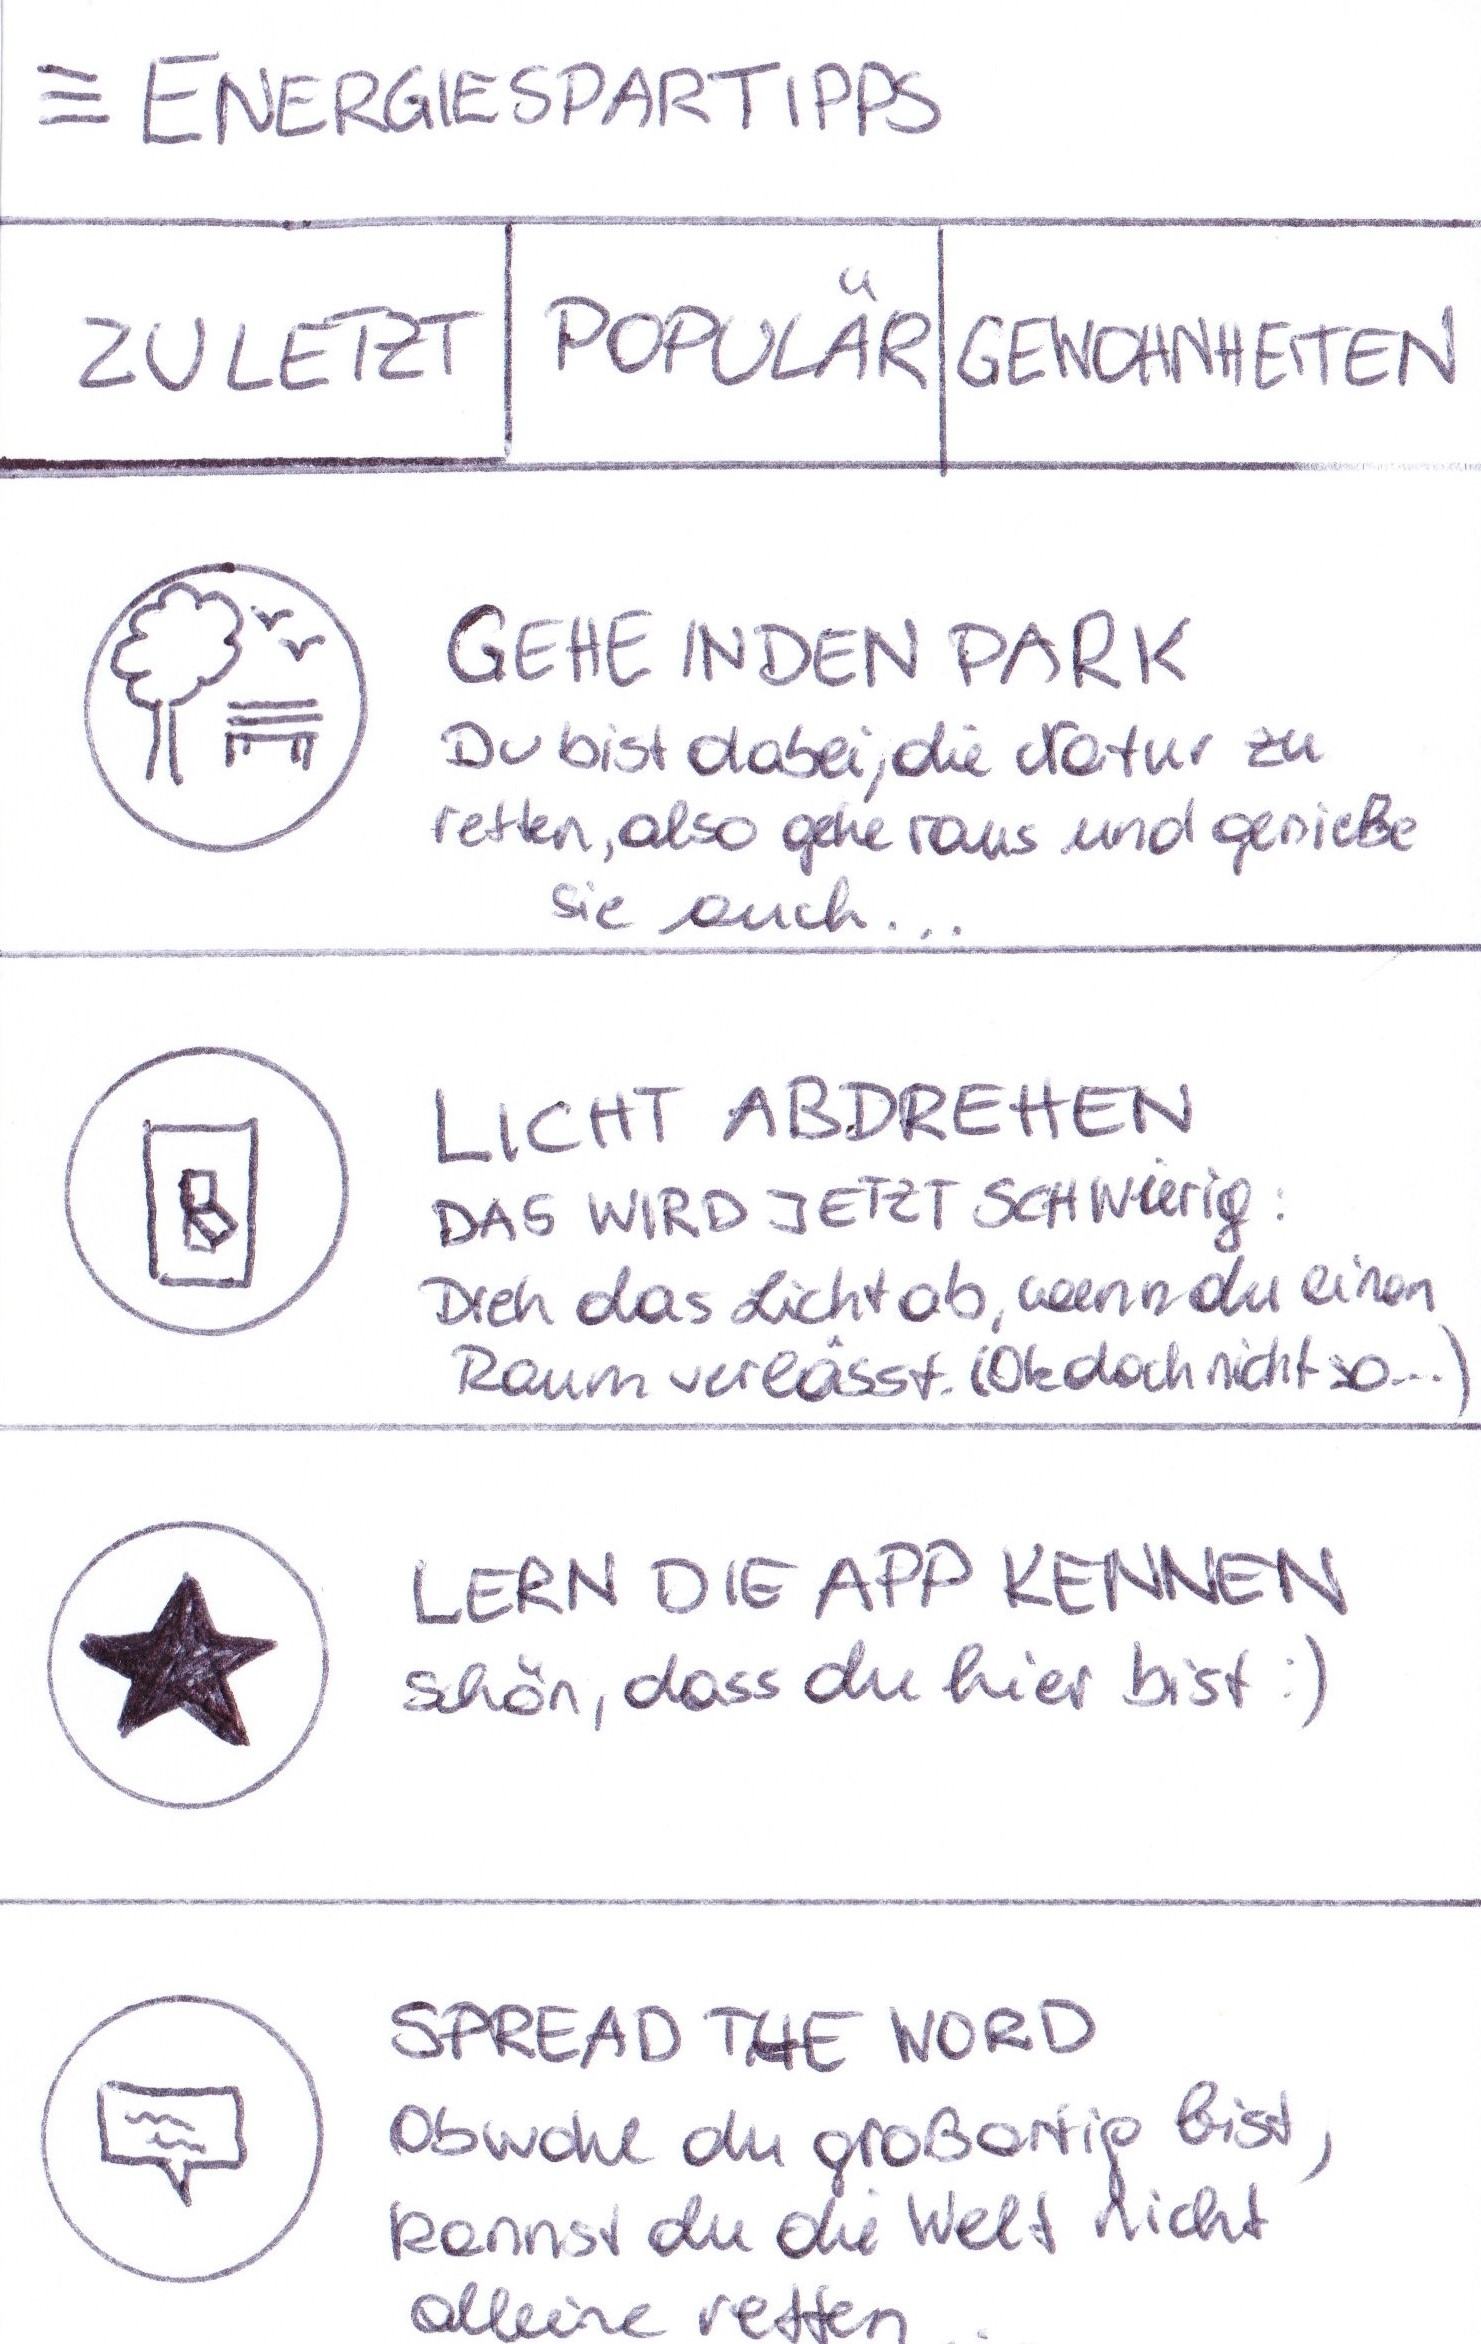
\includegraphics[width=\textwidth]{screens/tipp_4}
		\subcaption{Hedonist}
		\label{fig:tipps:hedonist}
	\end{subfigure}
	\caption{The paper prototype screen for energy saving tips}
	\label{fig:tipps} % \label has to be placed AFTER \caption (or \subcaption) to produce correct cross-references.
\end{figure}

\begin{figure}[h]
	\centering
	\begin{subfigure}[b]{0.24\columnwidth}
		\centering
		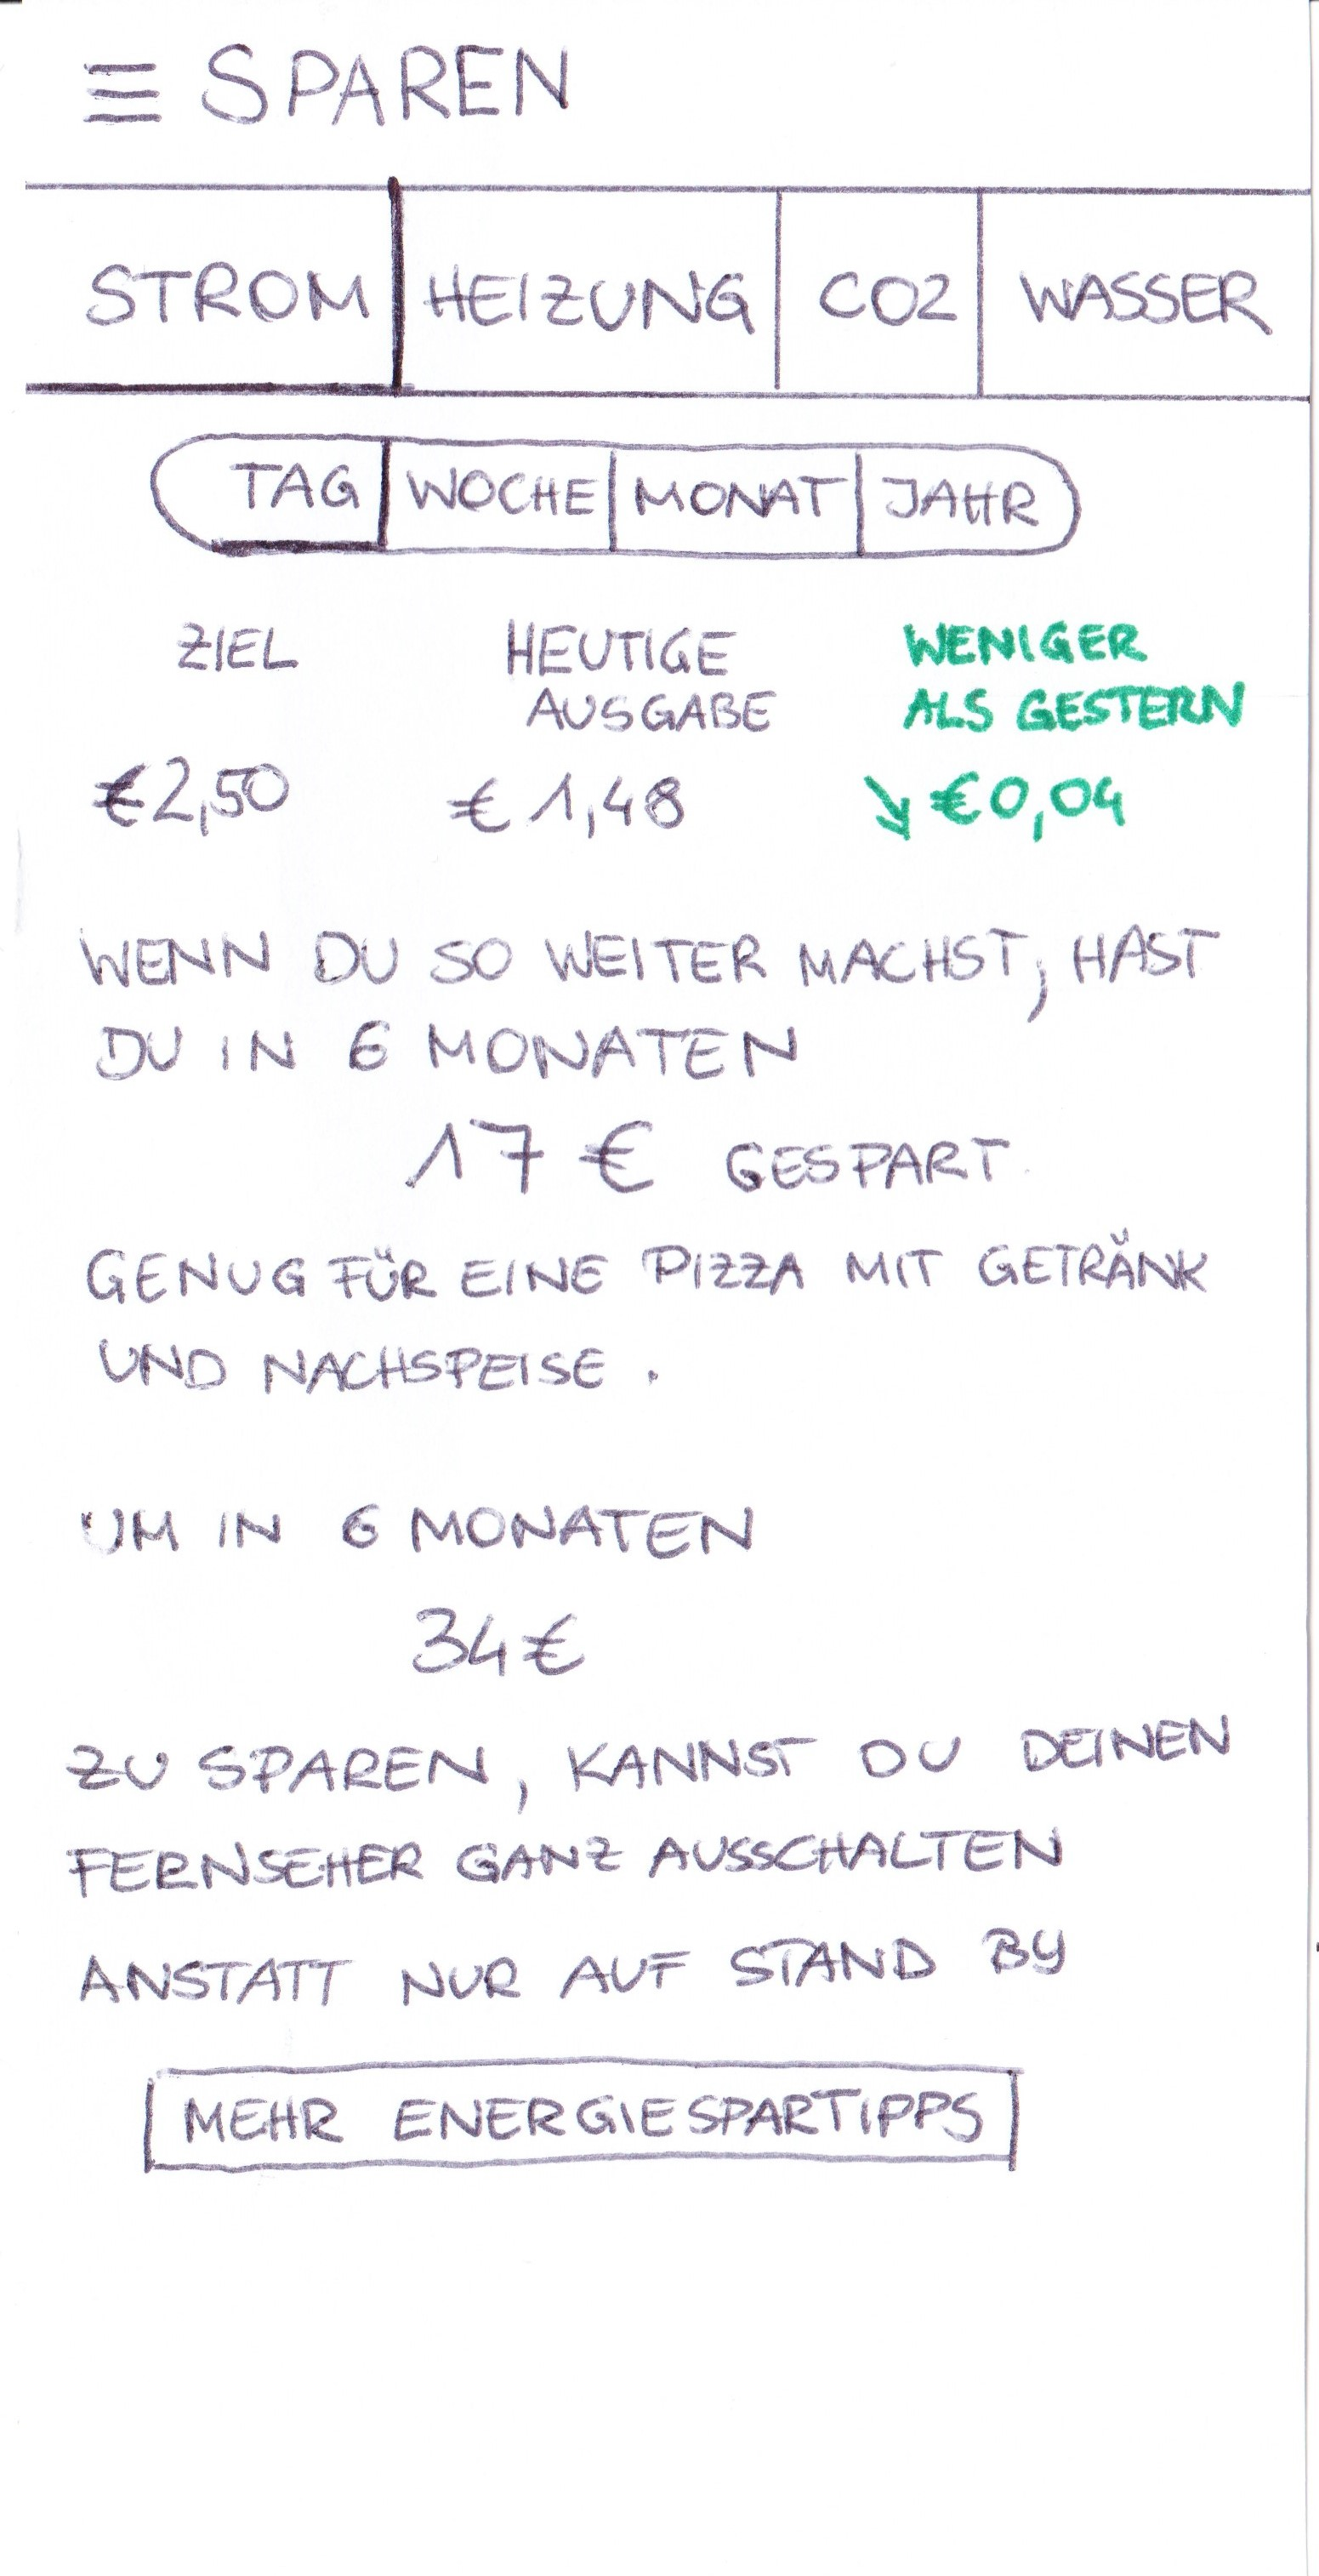
\includegraphics[width=\textwidth]{screens/Sparen_1}
		\subcaption{Professional}
		\label{fig:sparen:professional}
	\end{subfigure}
	\begin{subfigure}[b]{0.24\columnwidth}
		\centering
		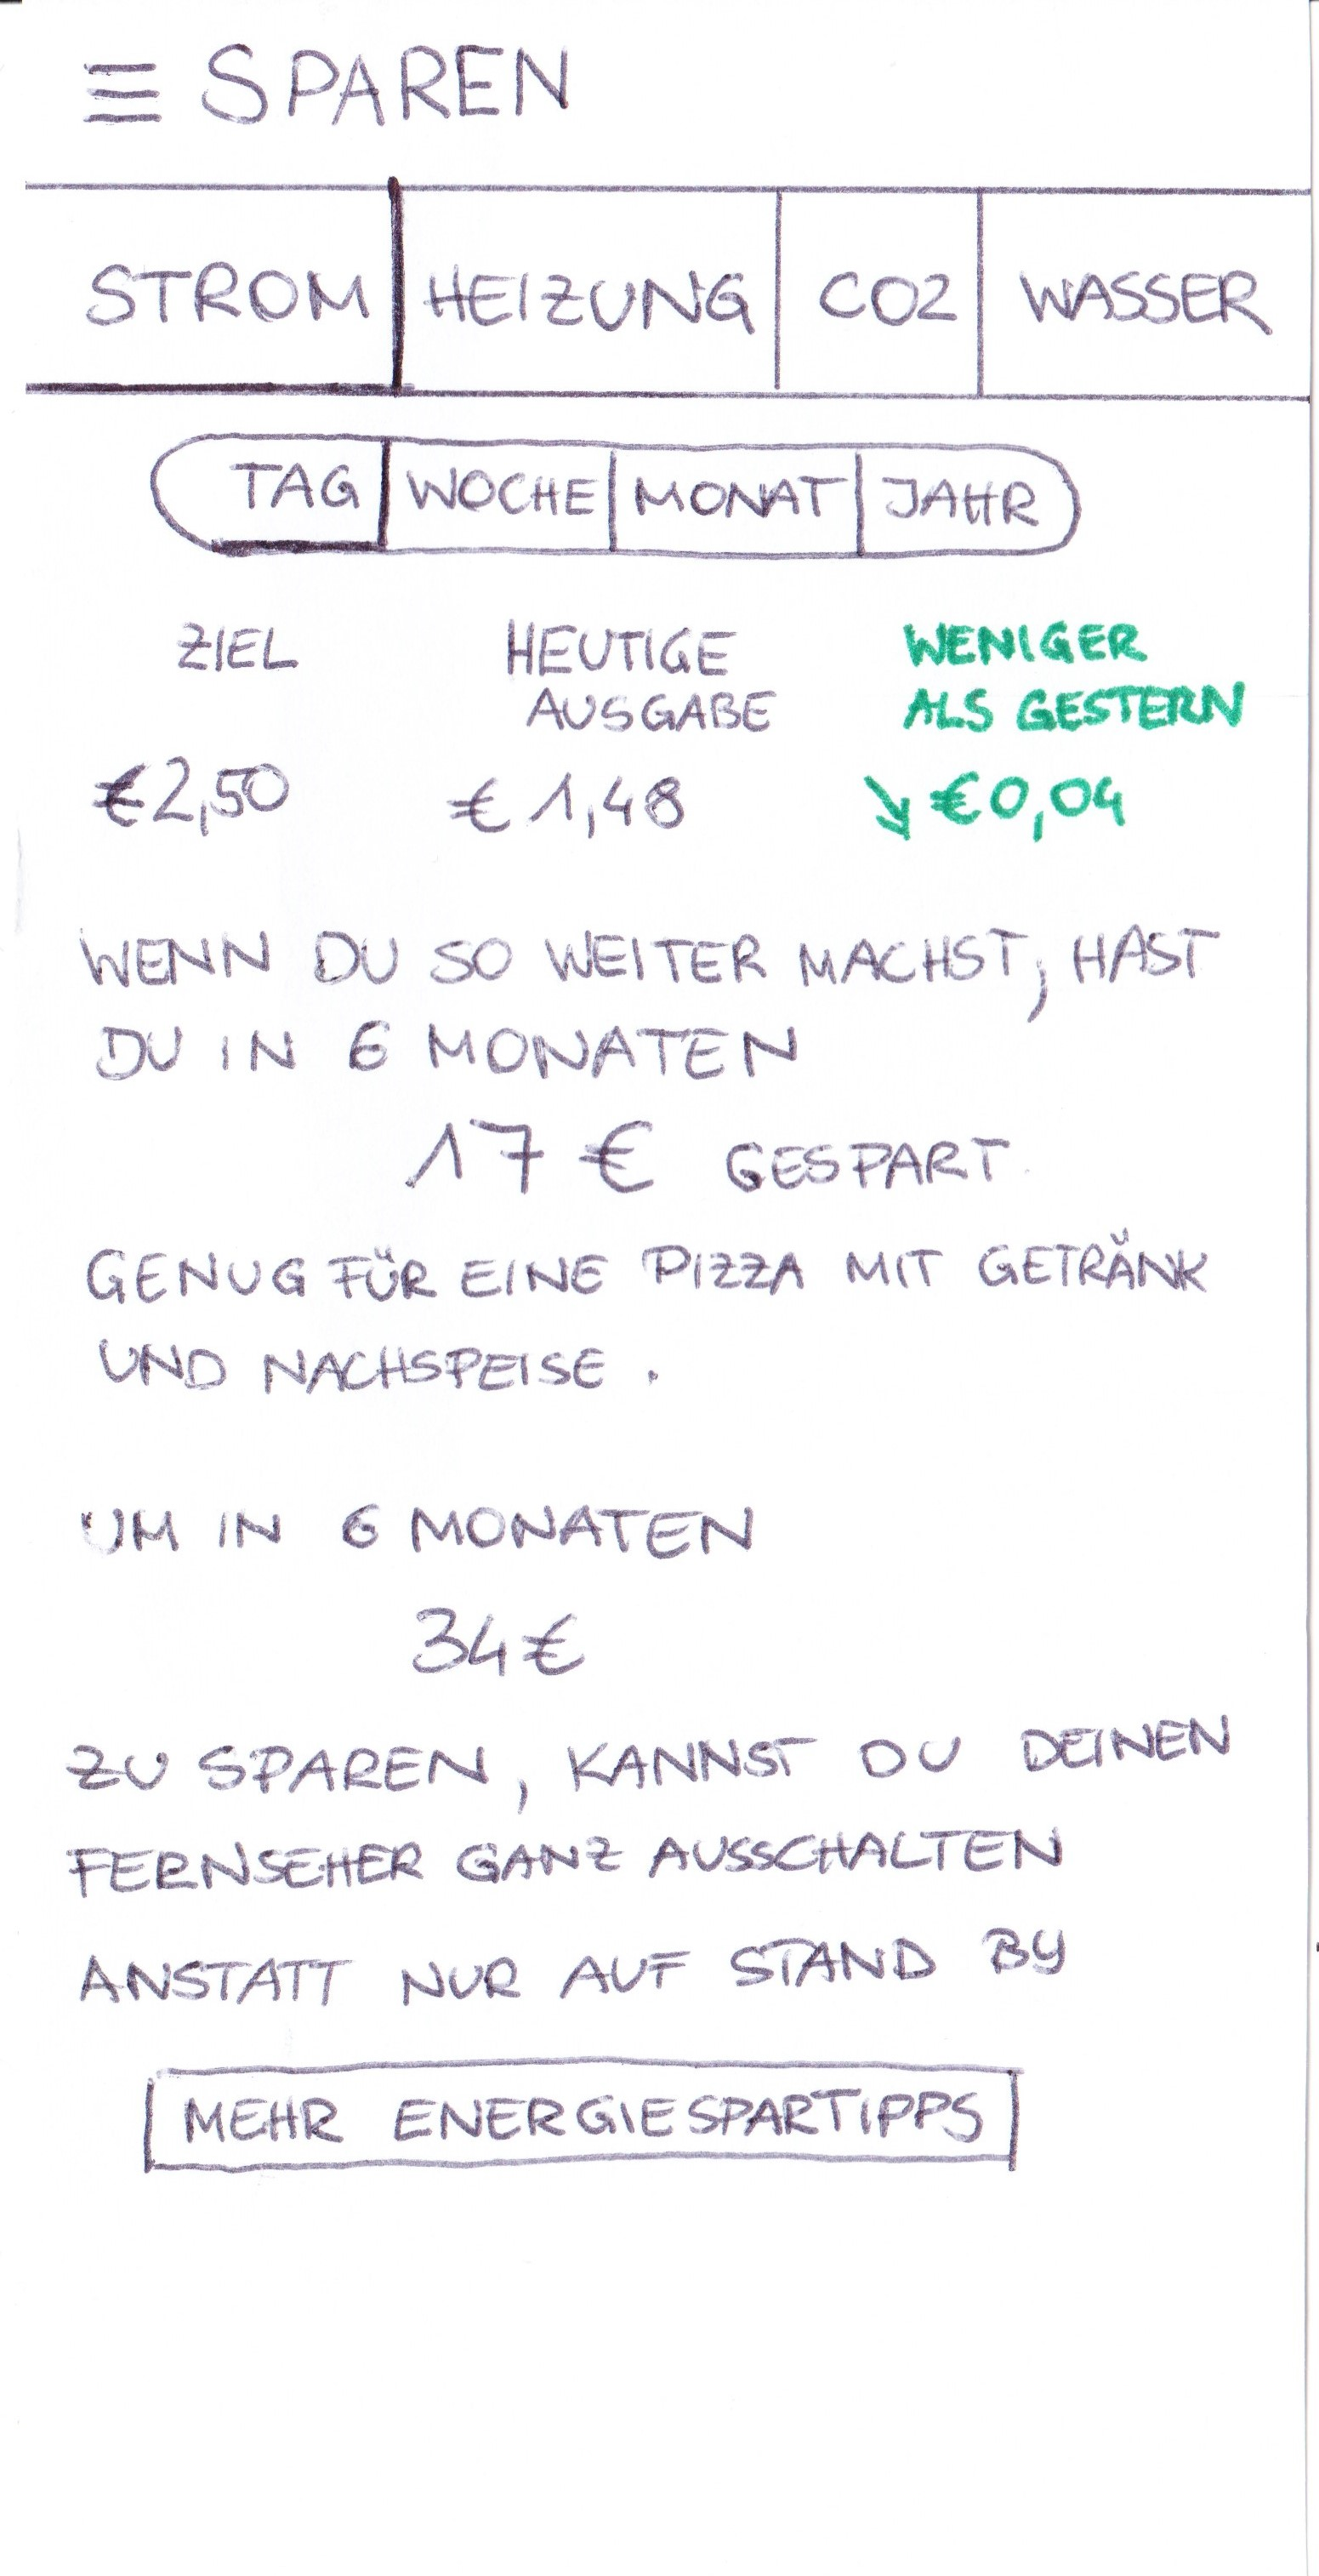
\includegraphics[width=\textwidth]{screens/Sparen_2}
		\subcaption{Optimizer}
		\label{fig:sparen:optimizer}
	\end{subfigure}
	\begin{subfigure}[b]{0.24\columnwidth}
		\centering
		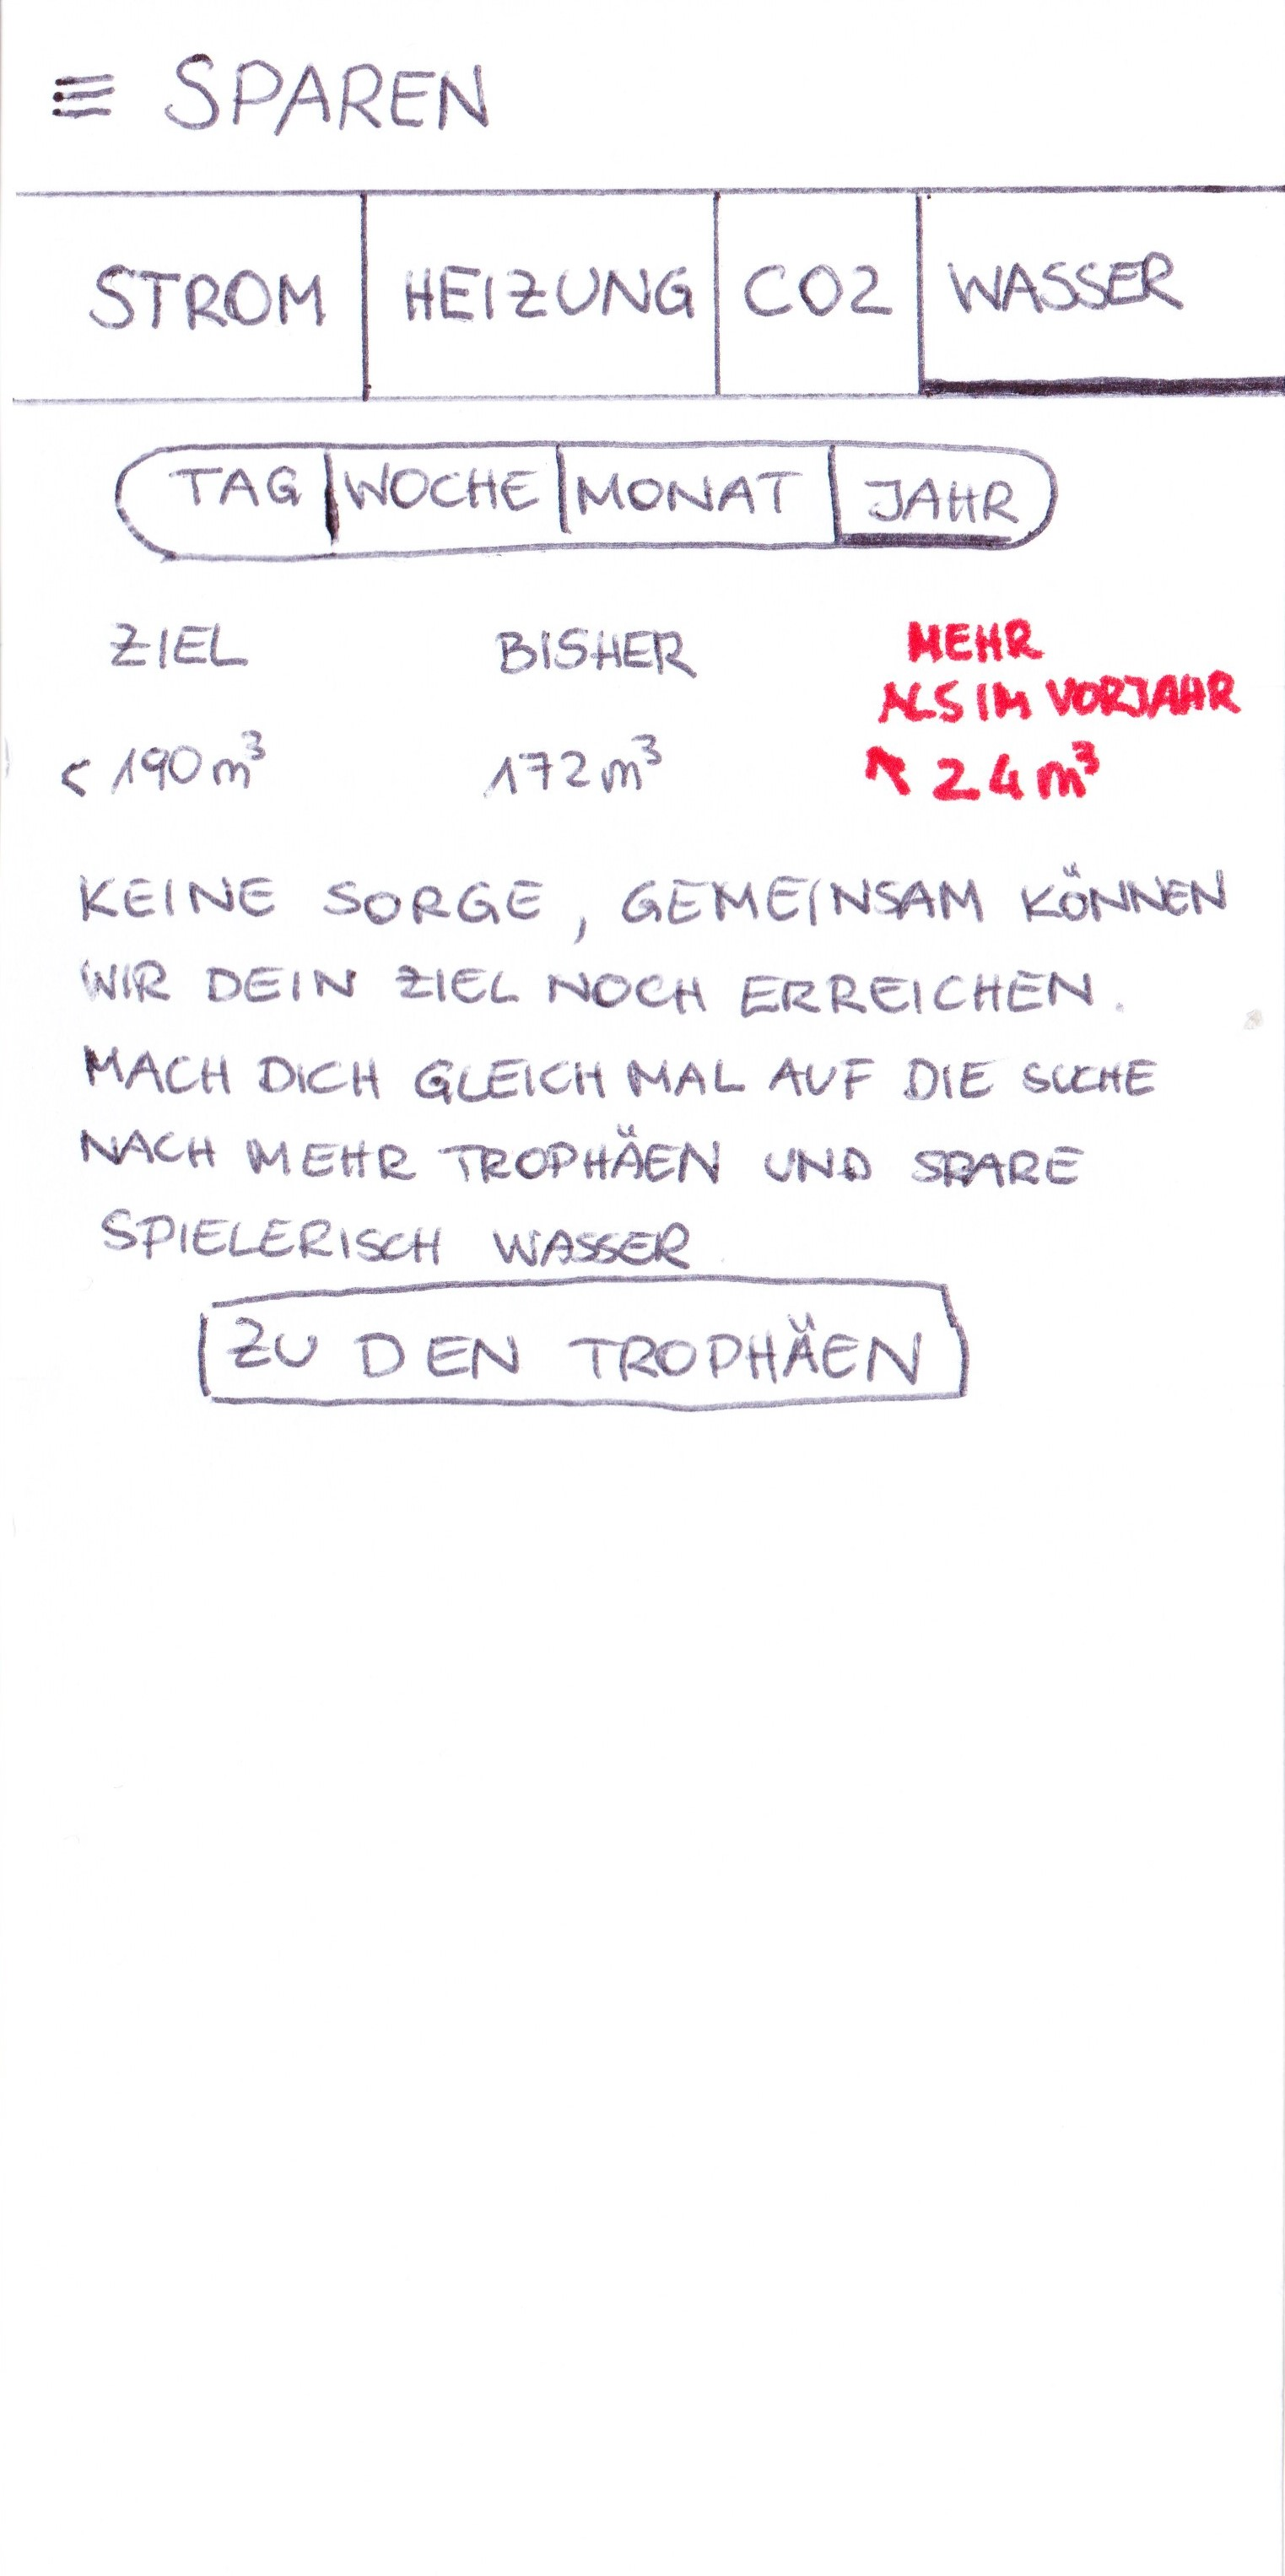
\includegraphics[width=\textwidth]{screens/Sparen_3}
		\subcaption{Indifferent}
		\label{fig:sparen:indifferent}
	\end{subfigure}
	\begin{subfigure}[b]{0.24\columnwidth}
		\centering
		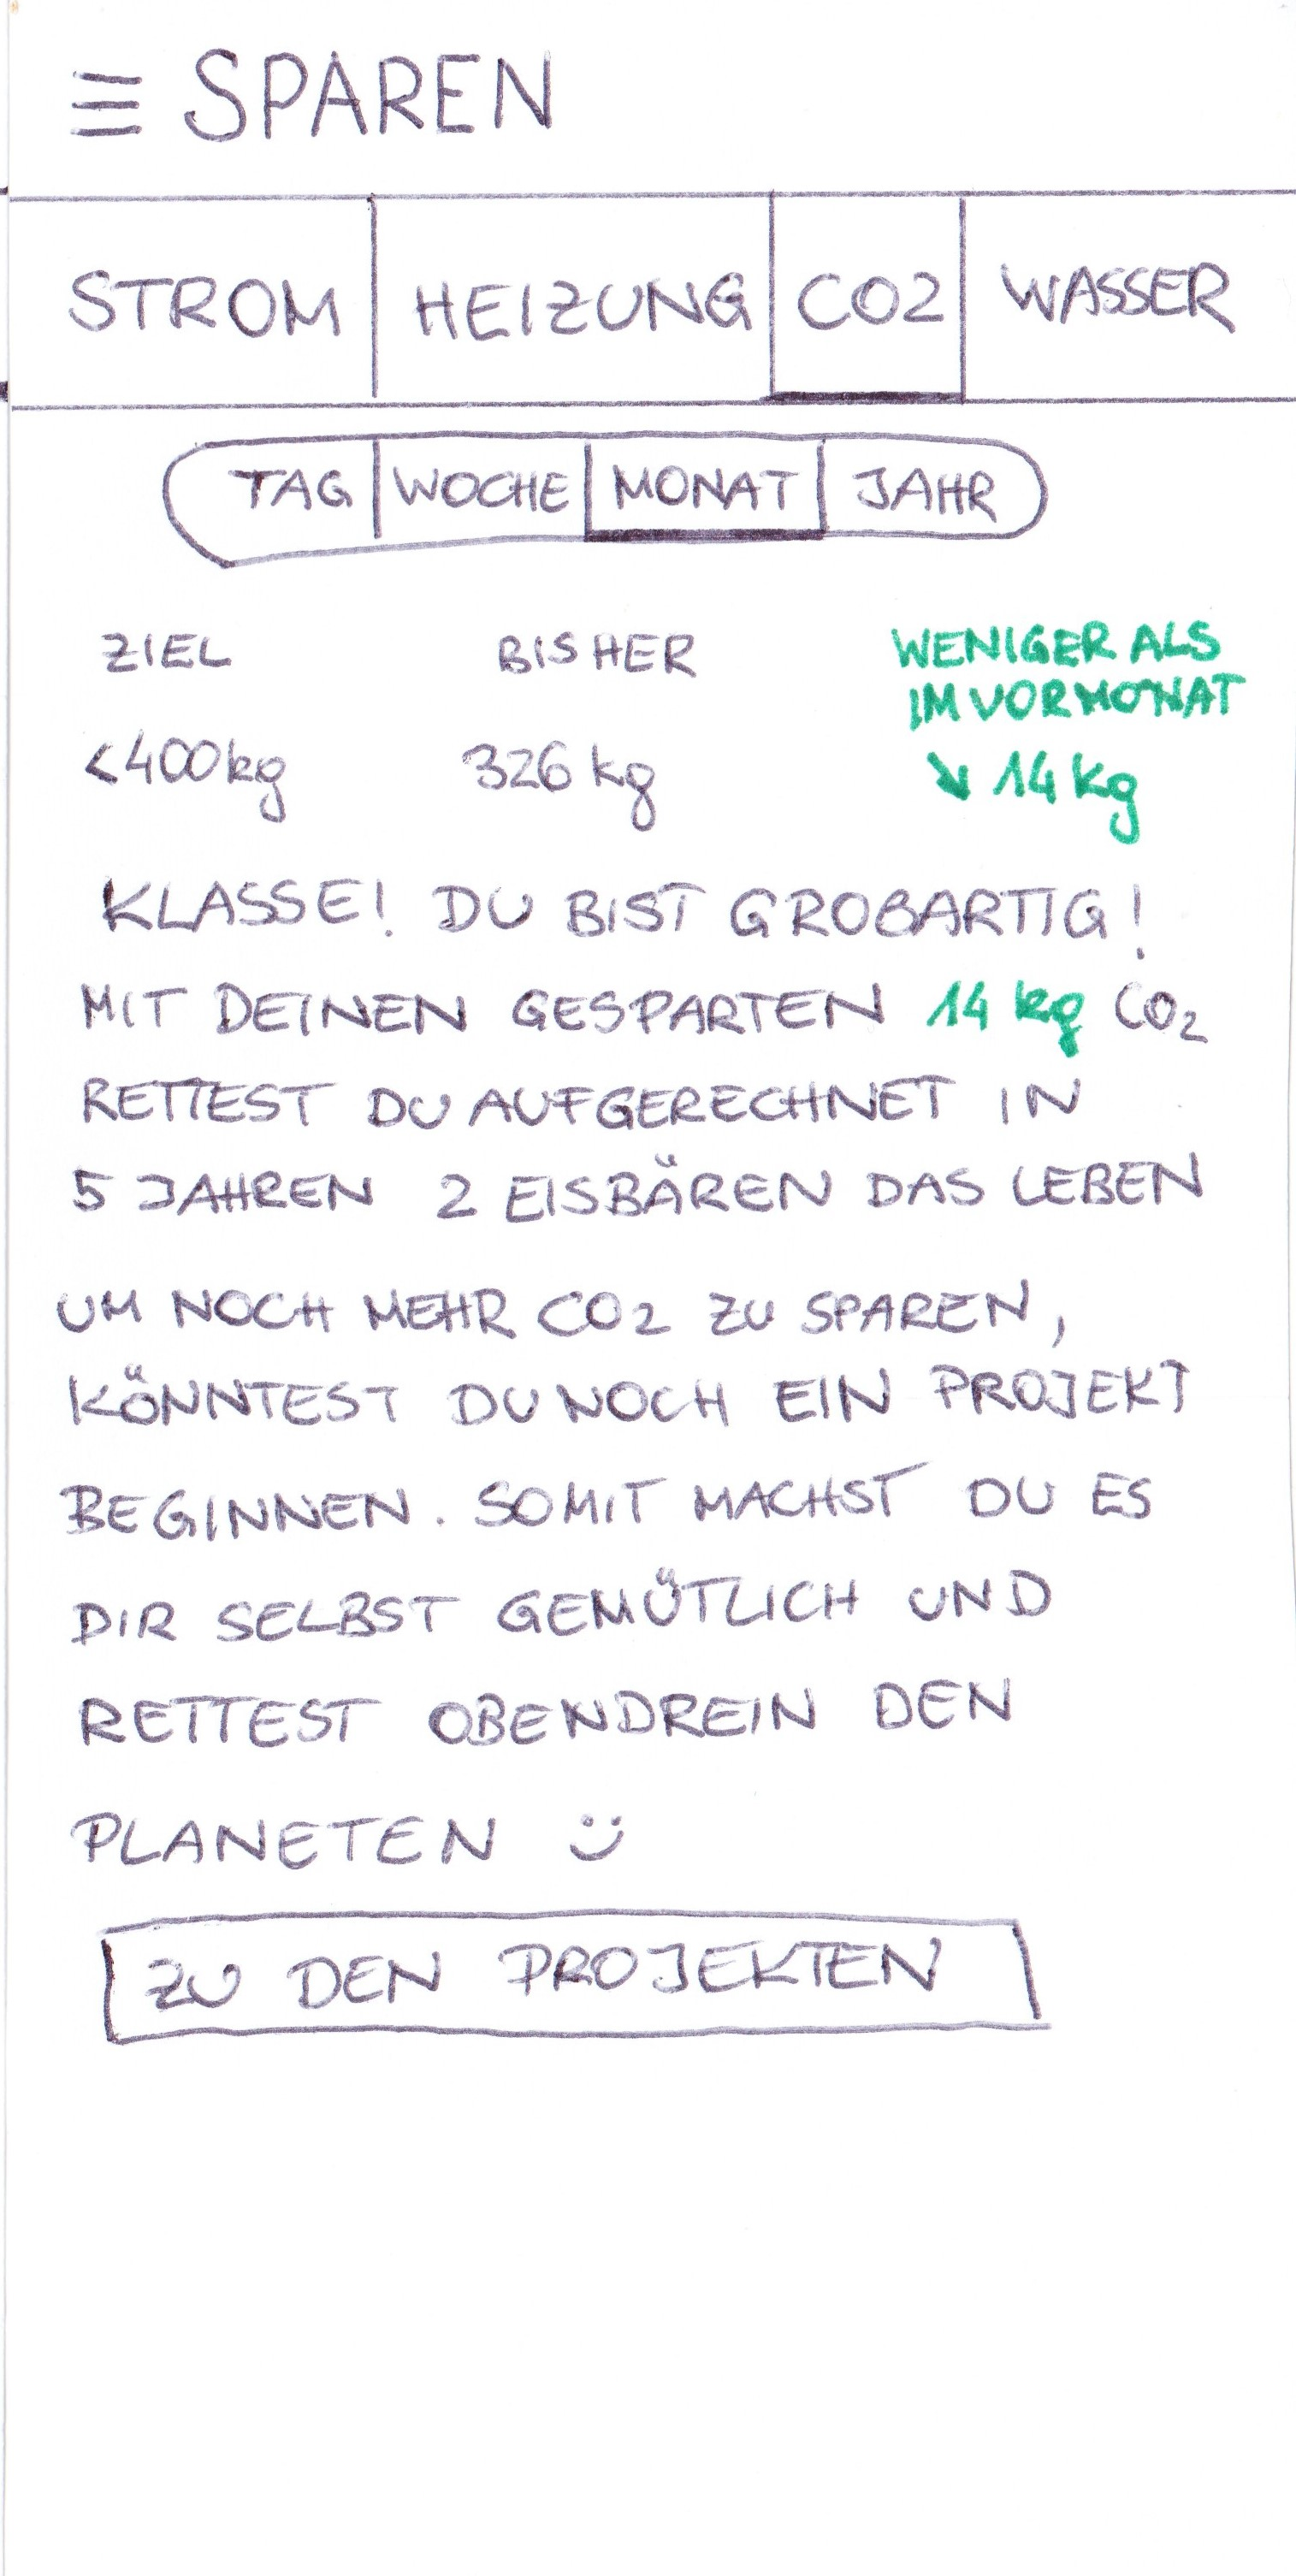
\includegraphics[width=\textwidth]{screens/Sparen_4}
		\subcaption{Hedonist}
		\label{fig:sparen:hedonist}
	\end{subfigure}
	\caption{The paper prototype screen for saving}
	\label{fig:sparen} % \label has to be placed AFTER \caption (or \subcaption) to produce correct cross-references.
\end{figure}

\begin{figure}[h]
	\centering
	\begin{subfigure}[b]{0.24\columnwidth}
		\centering
		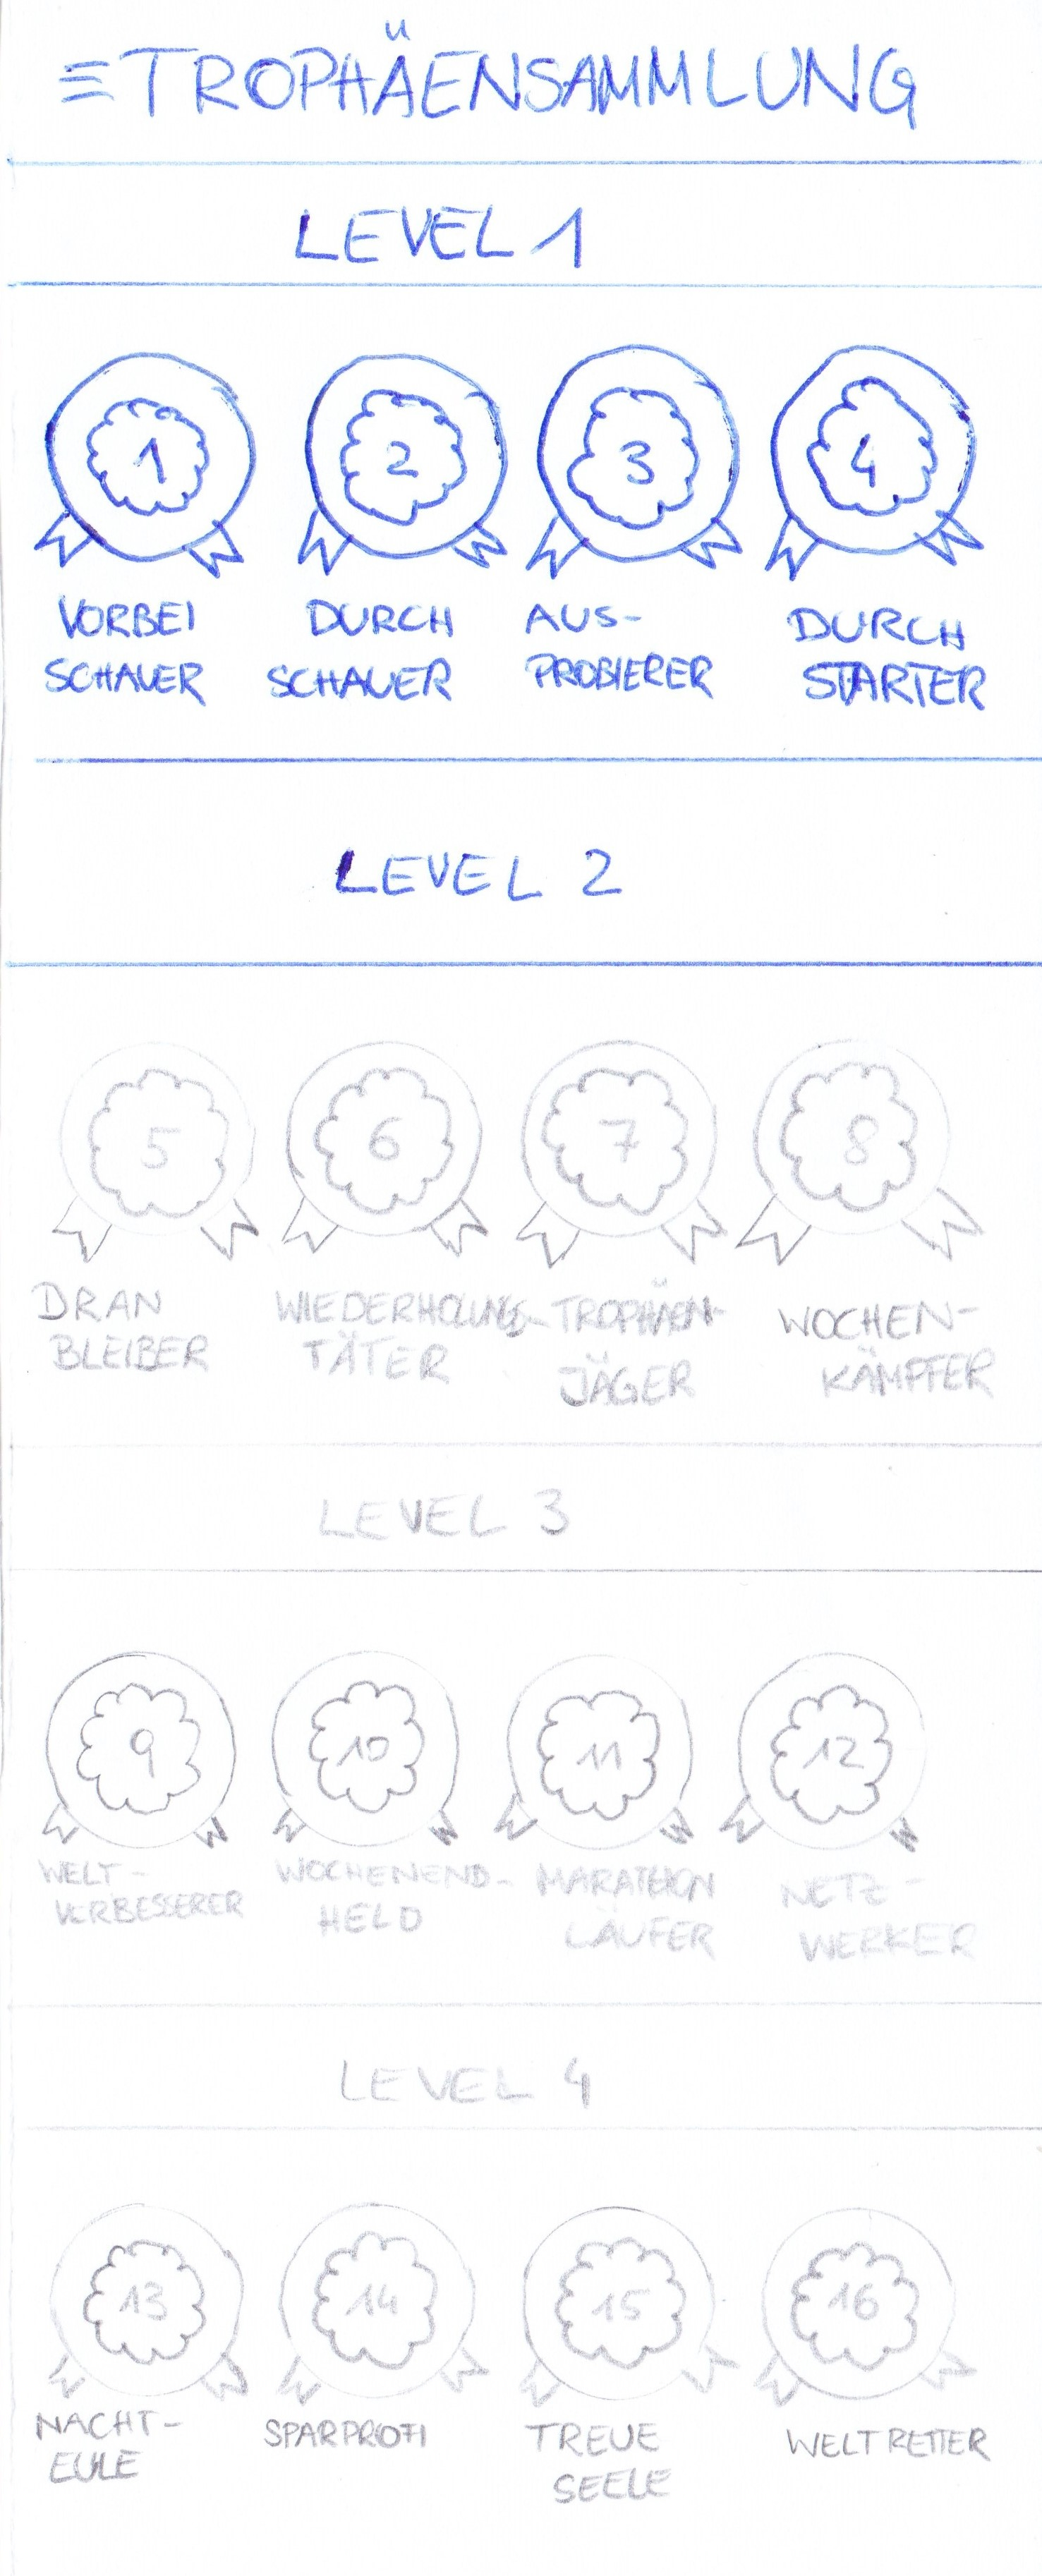
\includegraphics[width=\textwidth]{screens/Trophaensammlung}
		\subcaption{Professional and Hedonist}
		\label{fig:trophaen}
	\end{subfigure}
	\begin{subfigure}[b]{0.24\columnwidth}
		\centering
		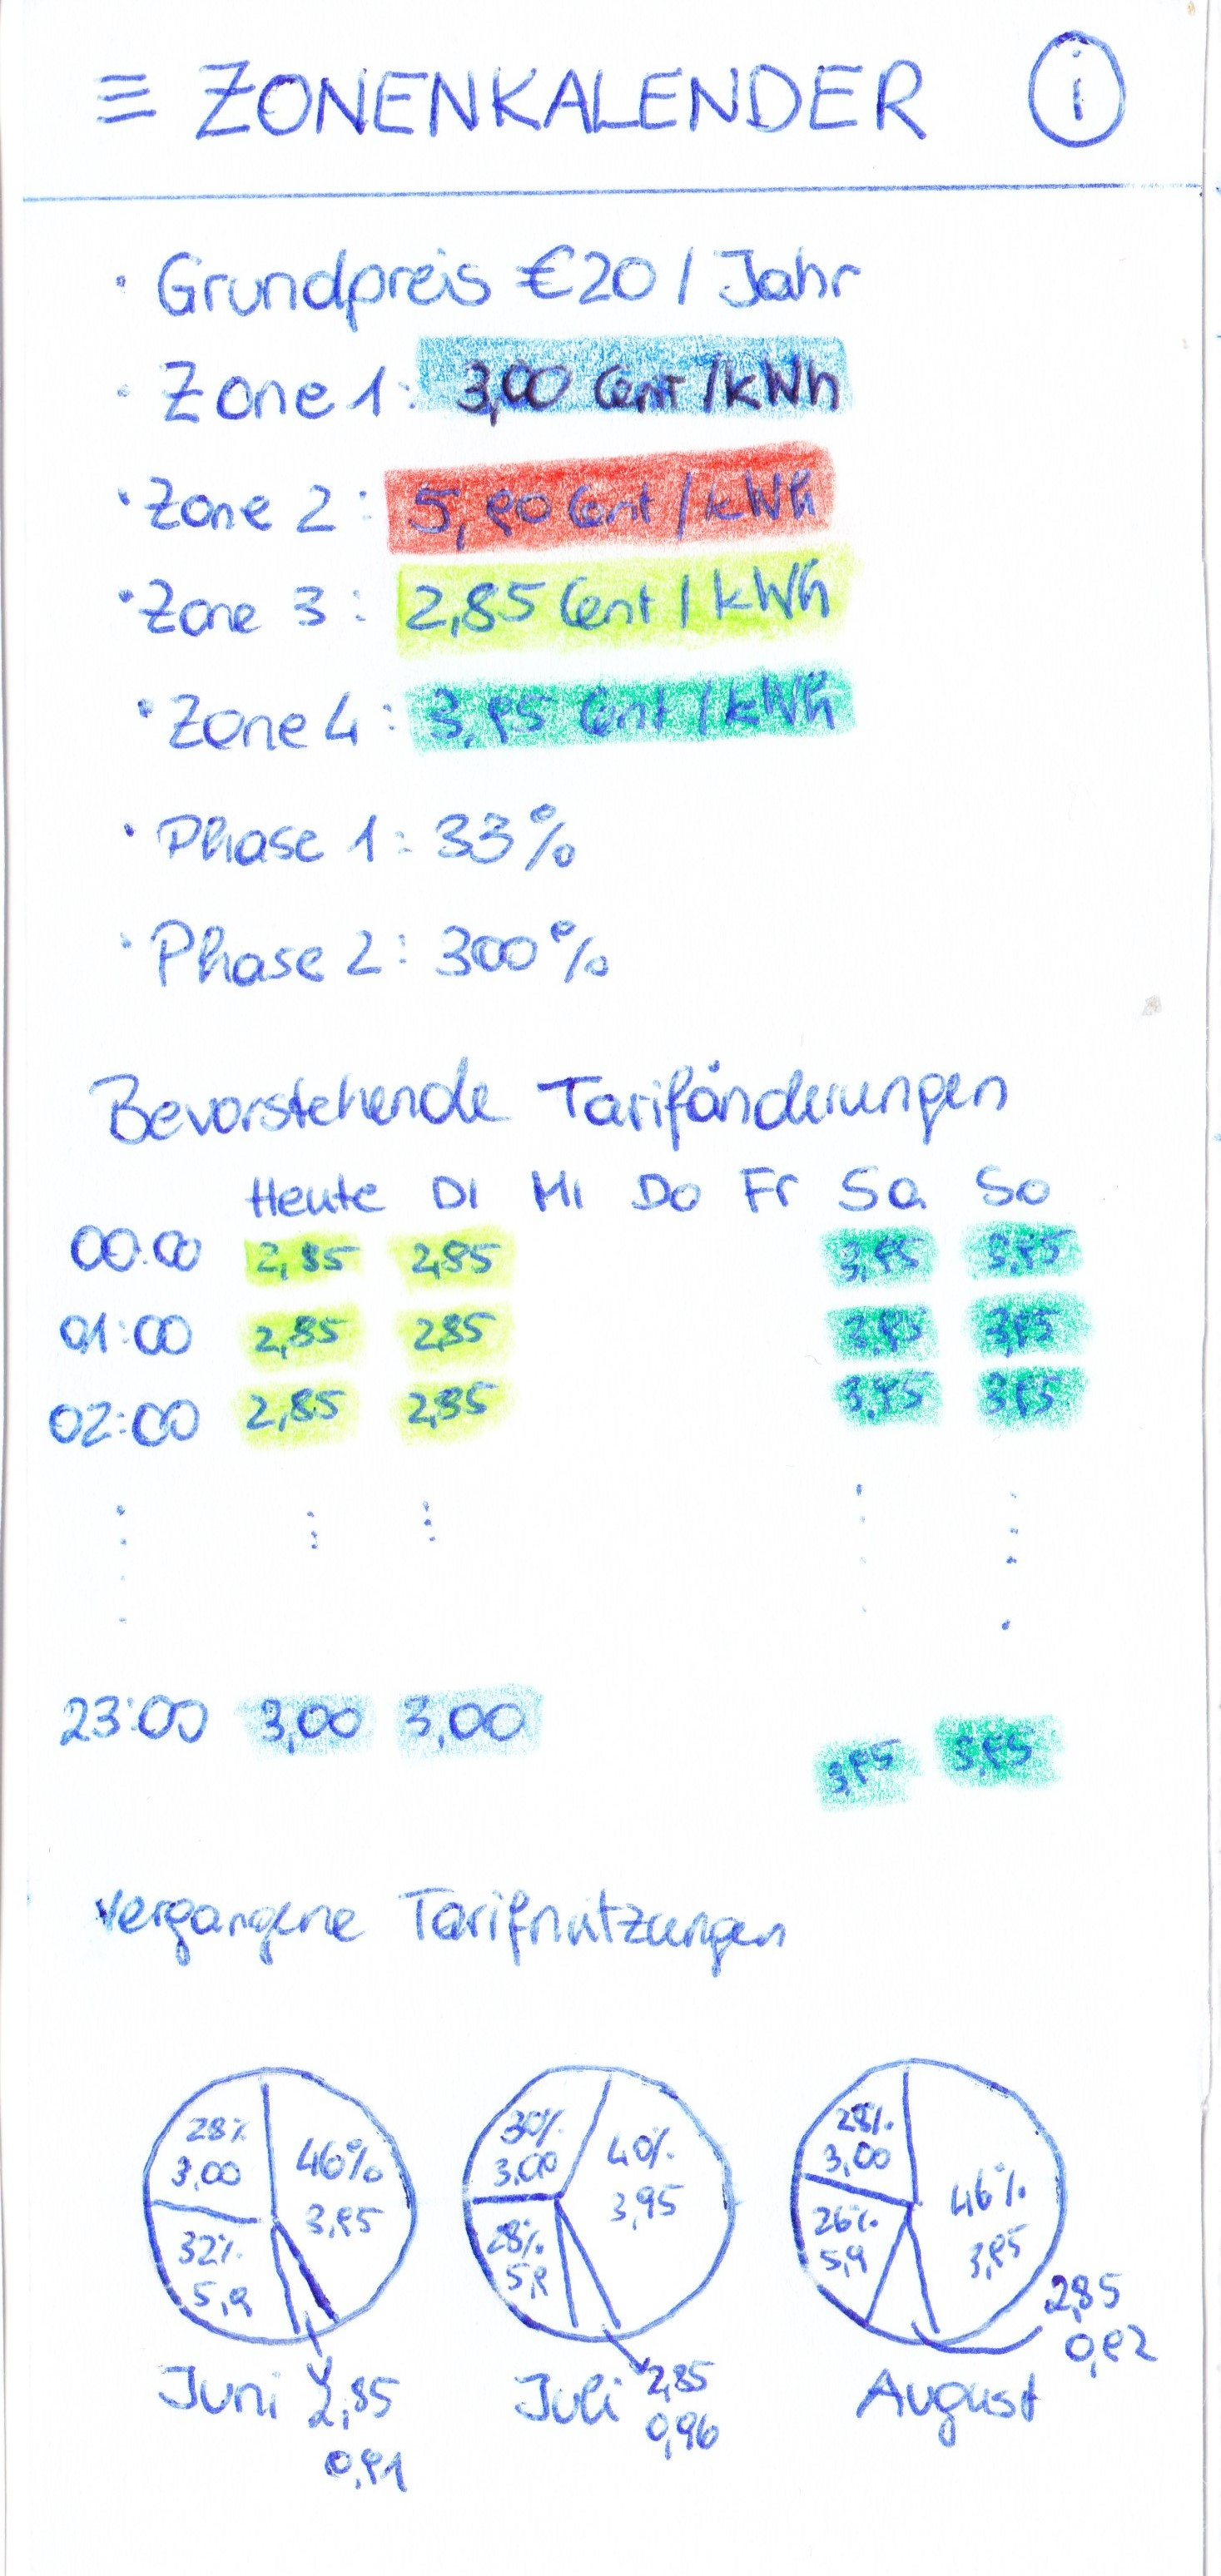
\includegraphics[width=\textwidth]{screens/Zonenkalender}
		\subcaption{Optimizer and Indifferent}
		\label{fig:zonen:optimizer}
	\end{subfigure}
	\caption{The proposed screens for statistics}
	\label{fig:kalender-} % \label has to be placed AFTER \caption (or \subcaption) to produce correct cross-references.
\end{figure}


\section{Recommendations for improvement for the ASCR App}

